\documentclass[article,A4,11pt]{llncs}
\usepackage[T1]{fontenc}
\usepackage{amsmath}
\usepackage{amssymb}

\usepackage{epsf,times}
\usepackage{amsfonts}
\usepackage{graphicx}
\usepackage{mathrsfs}
\usepackage{wrapfig}

\usepackage{color}
\usepackage{amsmath,mathrsfs,bm}
\usepackage{cases}
\usepackage{subfig}
\usepackage{multicol}
\usepackage{tabularx}

% DIMIER
\usepackage[T1]{fontenc}
%\newcommand{\tmname}[1]{\textsc{#1}}
%\newcommand{\tmop}[1]{\ensuremath{\operatorname{#1}}}
%\newcommand{\tmsamp}[1]{\textsf{#1}}
%\newcommand{\tmtextsc}[1]{{\scshape{#1}}}
%\newcommand{\tmtextsl}[1]{{\slshape{#1}}}
%\newcommand{\tmtexttt}[1]{{\ttfamily{#1}}}

\leftmargin=0.2cm
\oddsidemargin=1.2cm
\evensidemargin=0cm
\topmargin=0cm
\textwidth=15.5cm
\textheight=21.5cm
\pagestyle{plain}
\setlength{\columnsep}{20pt}

\def\m{\mathbf{m}}
\def\H{\mathbf{H}}
\def\E{\mathbf{E}}
\newcommand{\vepsi}{{\varepsilon}}
\def\hnorm#1#2{\vert\,#1\,\vert_{#2}}
\newcommand{\R}{{\mathbb R}}
\newcommand{\Sph}{{\mathbb S}}
\def\x{\mathbf{x}}
\def\hvec{\overline{\mathbf{h}}}
\def\evec{\overline{\mathbf{e}}}

\DeclareMathAlphabet{\mathpzc}{OT1}{pzc}{m}{it}
%\leftmargin=0cm
%\oddsidemargin=1cm
%\textwidth=14cm
%\pagestyle{plain}

\newcommand{ \etal}{\mbox{\emph{et al. }}}

\newcommand\vect[1]{\mbf{#1}}
\newcommand{\mbf}[1]{\mbox{\boldmath$#1$}} 
\newcommand{\RC}[1]{#1 $\times$ #1 $\times$ #1}
\def\um{$\mu$m}
\def\C{$^{\circ}\mathrm{C}$}

\newcommand{\Rmnum}[1]{\expandafter\@slowromancap\romannumeral #1@}

\def\clovek#1{\noindent\bgroup\vbox{\noindent#1}\egroup\vskip1em}

% DEFINITION OF CUSTOM FONT SIZE
\newcommand{\customfontA}{\fontsize{50}{55}\selectfont}
\newcommand{\customfontB}{\fontsize{14.4}{20}\selectfont}
\newcommand{\customfontC}{\fontsize{30}{35}\selectfont}

% TO INPUT BACKGROUND IMAGE
\usepackage{eso-pic}
\newcommand\BackgroundPic{
\put(0,0){
\parbox[b][\paperheight]{\paperwidth}{
\vfill
\centering
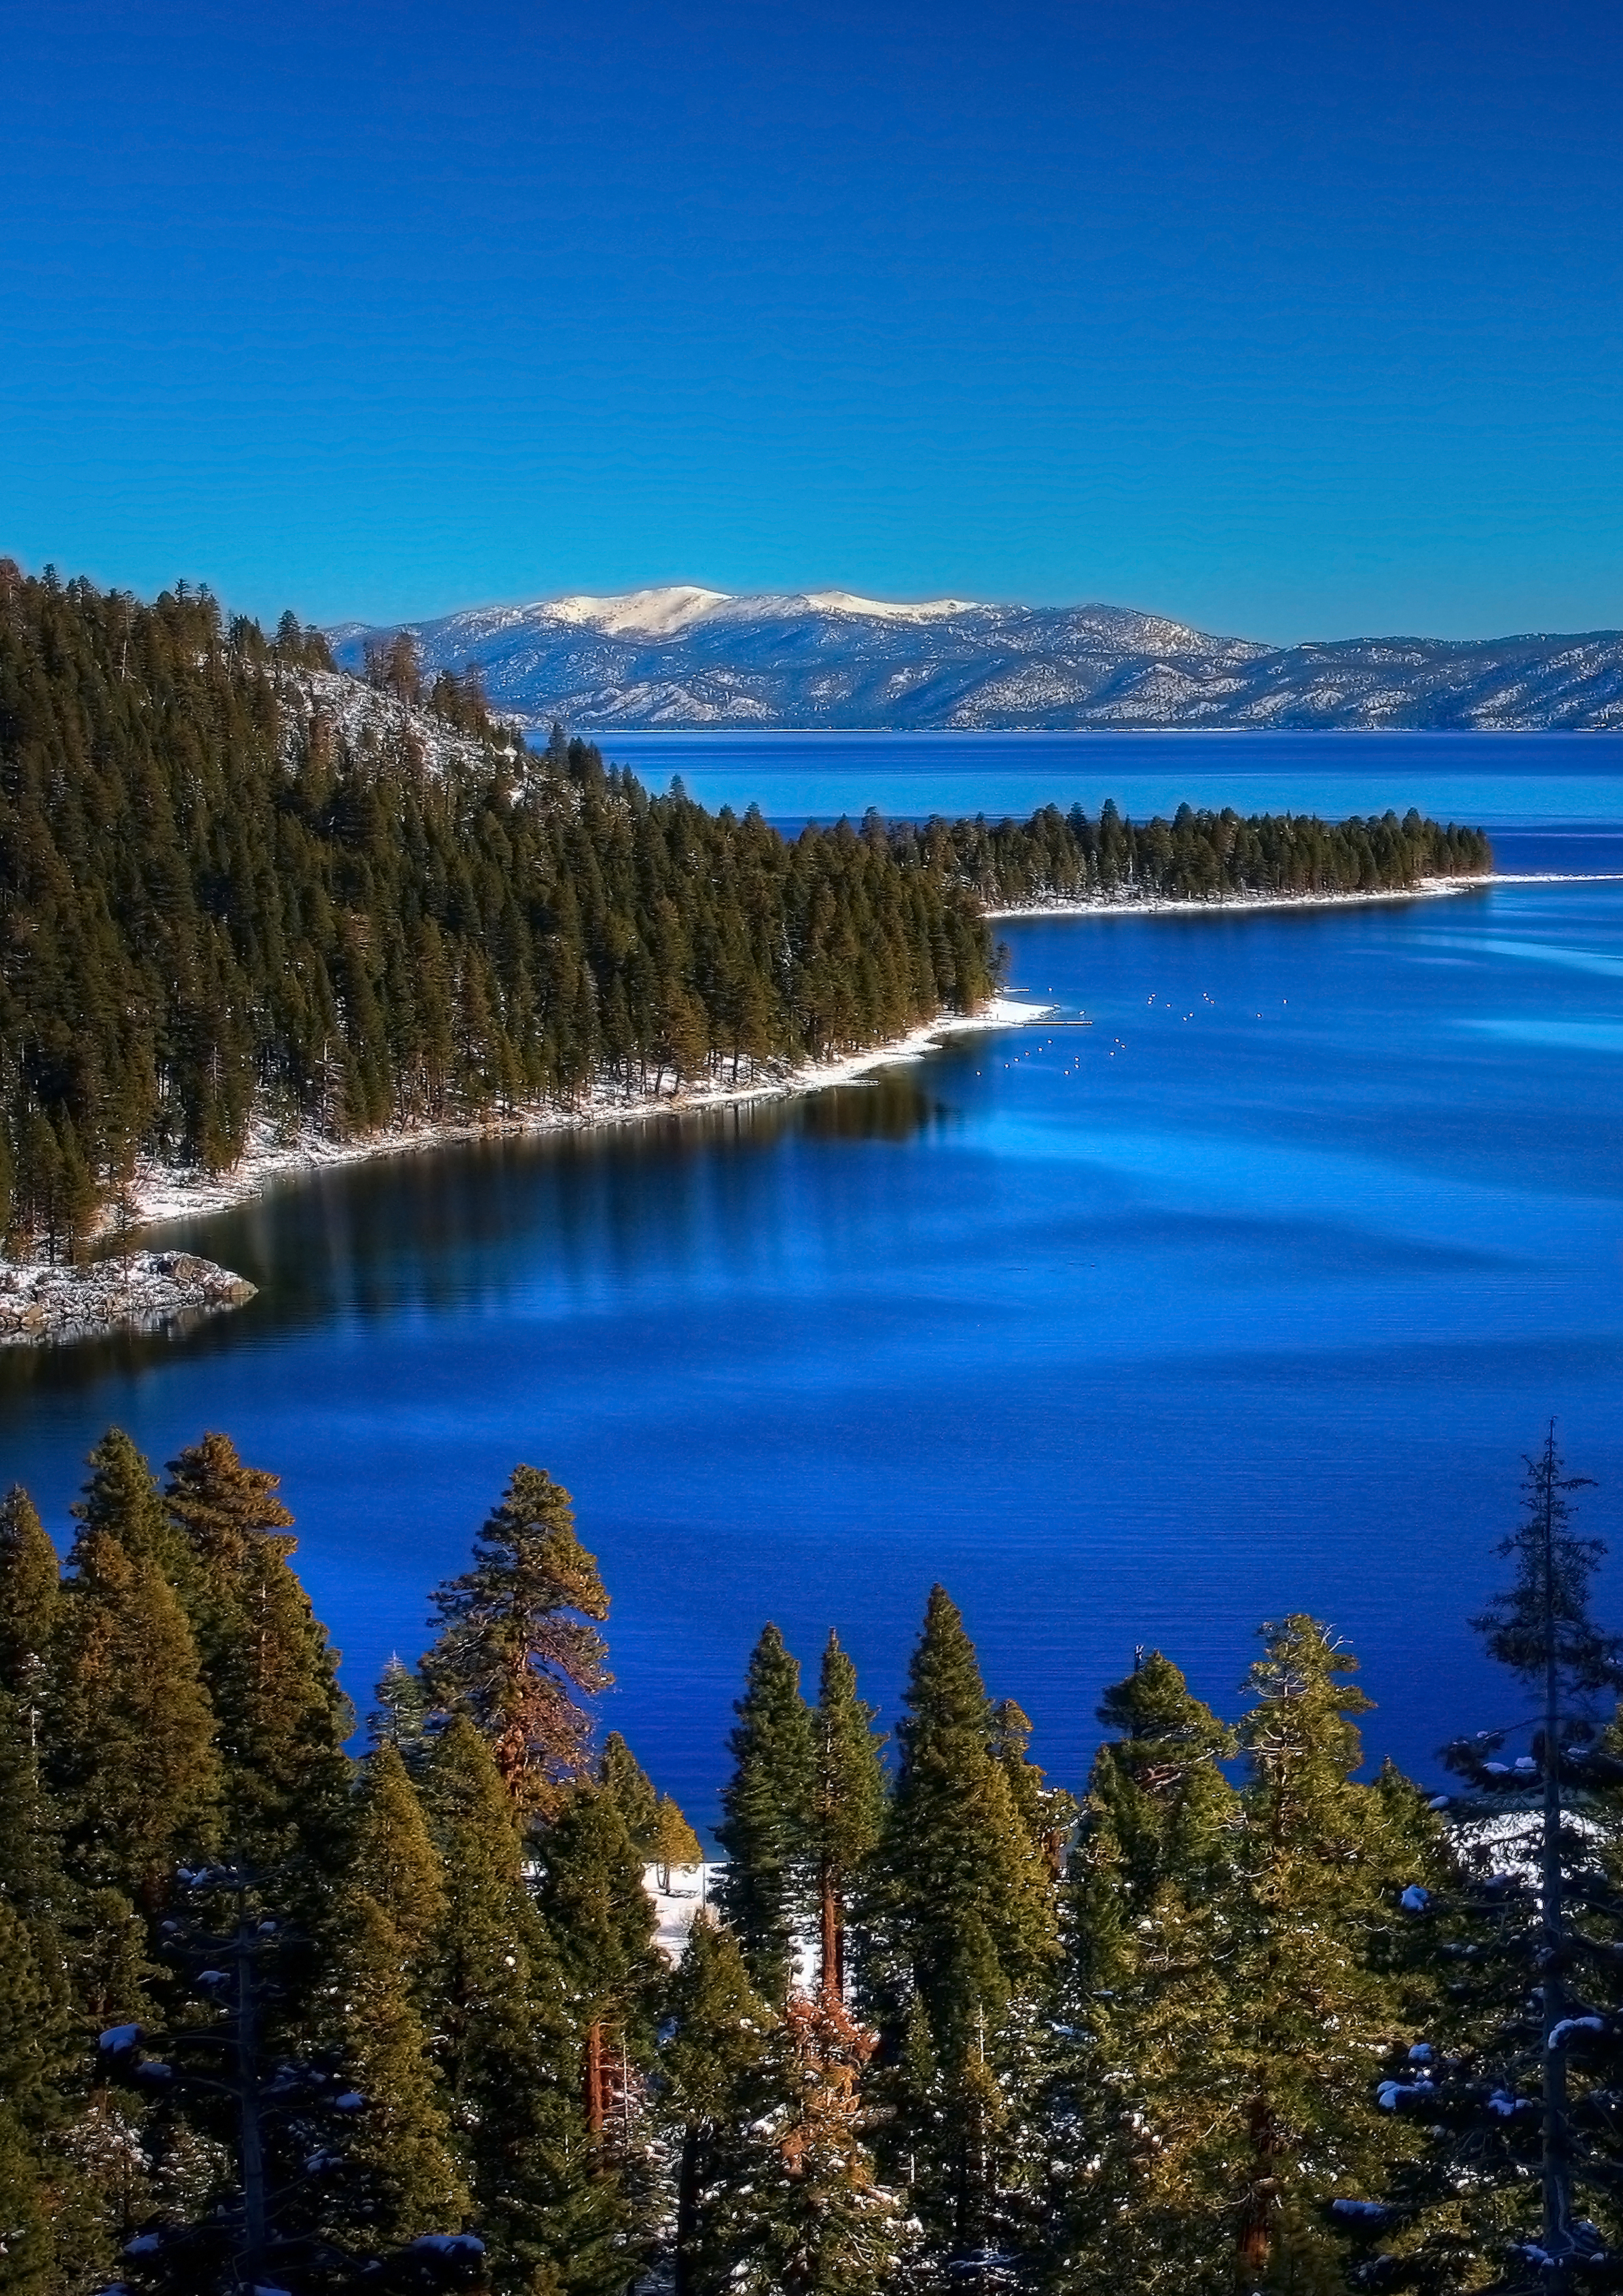
\includegraphics[width=\paperwidth,height=\paperheight]{background.png}
\vfill
}}}

\begin{document}

% INPUTTING BACKGROUND IMAGE
\AddToShipoutPicture{\BackgroundPic}

\vbox{}
\pagestyle{empty}

\newpage

\textwidth=15.5cm

\ClearShipoutPicture

\newpage

\section*{}

\vspace*{60mm}
ISBN ???-??-????-???-?\\ \\
This is a joint publication of the 
University of Nevada (Reno), 
Desert Research Institute (Reno),
Idaho National Laboratory (Idaho Falls),
U.S. Army R\&D Center (Vicksburg), 
Institute of Thermomechanics (Prague, Czech Republic), 
and University of West Bohemia (Pilsen, Czech Republic).\\

\noindent
FEMTEC 2011:
3rd International Conference on Computational Methods in Engineering and Science\\

\noindent
\begin{tabular}{ll}
Editors: & Pavel Solin (University of Nevada, Reno \& Institute of Thermomechanics, Prague) \\
 & Glen Hansen (Idaho National Laboratory)\\
 & Pavel Karban (University of West Bohemia, Pilsen) \\
 & Chris Kees (U.S. Army R\&D Center, Vicksburg, Mississippi) \\
 & Darko Koracin, Matt Reeves (Desert Research Institute, Reno) \\
Publisher: & University of Nevada, Reno \\
 & 1664 North Virginia Street \\
 & Reno, NV 89557 - 0084\\
 & U.S.A.\\
Printed by: & XXXXXXXXX \\
 & XXXXXXXXX\\
 & XXXXXXXXX\\
Year: & 2011\\
\end{tabular}

\subsection*{Contact Information}

Mailing address:\\
FEMTEC 2011 Conference\\
Department of Mathematics and Statistics\\
University of Nevada, Reno, NV 89557 - 0084\\ 

\noindent
E-mail: {\tt femtec2011@unr.edu}\\
Web page: {\tt http://hpfem.org/events/femtec-2011/}\\
Phone: 1-775-848-7892

\chapter*{\huge FEMTEC 2011}
\vspace{-5mm}
\normalsize   
\begin{center}
3rd International Conference on Computational Methods in Engineering and Science\\
Harvey's Casino and Resort\\ 
May 9 - 13, 2011\\
\end{center}
\vspace{-3mm}

\section*{Conference topics}

\begin{itemize}
  \item Computational methods in geosciences including, but not limited to, 
        atmospheric sciences (weather and climate), hydrology, geology, 
        atmospheric chemistry, air pollution, and related disciplines. 
  \item Computational methods in nuclear, mechanical, civil, electrical, and 
        other engineering fields. 
  \item Mesh generation and scientific visualization. 
  \item Open-source scientific computing software.
  \item Interactive browser tools, web-based computing and visualization.
  \item Python in open source scientific computing projects.
  \item Novel scientific computing tools such as SciPy, NumPy, SymPy etc.
  \item Common platforms for scientific computing, interfacing and interoperability.
\end{itemize}

\subsection*{Scientific Committee}

\begin{itemize}
\item Valmor de Almeida (Oak Ridge National Laboratory, Oak Ridge, USA)
\item Ivo Dolezel (Czech Technical University, Prague, Czech Republic)
\item Glen Hansen (Idaho National Lab, Idaho Falls, USA)
\item Pavel Karban (University of West Bohemia, Pilsen, Czech Republic)
\item Christopher Kees (U.S. Army Engineer Research and Development Center, USA)
\item Matthew Knepley (University of Chicago, USA)
\item Darko Koracin (Desert Research Institute, Reno, USA)
\item Dmitri Kuzmin (University of Erlangen, Germany)
\item Stephane Lanteri (INRIA, France)
\item Matthias Moeller (Technical University of Dortmund, Germany)
\item Sascha Schnepp (Technical University of Darmstadt, Germany)
\item Stefan Turek (Technical University of Dortmund, Germany)
\item Gael Varoquaux (CEA Saclay, France)
\end{itemize}

\subsection*{Organizing Committee}

\begin{itemize}
\item Pavel Solin (University of Nevada, Reno and Institute of Thermomechanics, Prague)
\item Glen Hansen Idaho National Laboratory, Idaho Falls
\item Pavel Karban  (University of West Bohemia, Pilsen)
\item Christopher Kees U.S. Army Engineer R\& Center, Vicksburg
\item Darko Koracin, Matt Reeves, Desert Research Institute, Reno
\end{itemize}

\newpage
{\ }

\tableofcontents

%--------------------------------------------------------------------------------------
%--------------------------------------------------------------------------------------

\part{Abstracts of Keynote Lectures}

\pagestyle{plain}

\title{Finite Elements in Coastal Ocean Circulation Modeling}
\author{Clint Dawson} \institute{The University of Texas at Austin}

\begin{center}

\textbf{\Large Finite Elements in Coastal Ocean Circulation Modeling}\\
\vspace{10mm}
{\large Clint Dawson}\\
1 University Station, C0200 \\
The University of Texas at Austin \\
Austin, TX  78712 \\
{\tt clint@ices.utexas.edu}

\end{center}

\section*{Abstract}

Finite element methods of various types have been implemented by a number of researchers for modeling global and regional ocean circulation.  In this talk, we will discuss and compare two approaches investigated by the author and several collaborators for modeling circulation in the coastal ocean: a continuous Galerkin finite element method based on the generalized wave continuity equation (GWCE) \cite{LynchGray79}, and a discontinuous Galerkin (DG) formulation \cite{ad1,kub} based on the primitive form of the shallow water equations.

The GWCE is the basis for the Advanced Circulation (ADCIRC) model \cite{Luettich92}, which is a widely used quasi-operational shallow water simulator.    While this model has been shown to work well in many ``real-world'' situations, such as in modeling hurricane storm surges in the Gulf coast of the U.S. \cite{bunya,dietrich,MWR-Gustav}, it suffers from some drawbacks, including mass conservation errors, stability isues, and is restricted to low order approximations.  The DG formulation has certain potential advantages, including local mass conservation, the use of numerical fluxes and slope-limiters to prevent spurious oscillations, and the ability to use higher-order approximations locally within an element \cite{kub-p}.

We will compare both methods for standard model problems, examining both accuracy and parallel efficiency.  We will also discuss how features particular to coastal regions, such as wetting/drying and levees, are handled in each model. Finally, we will discuss results for both models  applied to actual hurricanes along the Gulf of Mexico coast, including Hurricane Ike, which hit Texas in 2008.  We will conclude with a discussion of current challenges and future research directions.

\bibliographystyle{plain}
\begin{thebibliography}{10}

\bibitem{LynchGray79} D. R. Lynch and W. R. Gray, A wave equation model for finite element computations, Computers and Fluids, 7, pp.\ 207-228, 1979.  

\bibitem{ad1} V.~Aizinger, C.~Dawson, A discontinuous Galerkin method for two-dimensional flow and transport in shallow water, Advances in Water Resources, 25, pp.\ 67-84, 2002

\bibitem{kub} E.J.~Kubatko, J.J.~Westerink, C.~Dawson, $hp$ Discontinuous Galerkin methods for advection dominated problems in shallow water flow, Comput.~Meth.~Appl.~Mech.~Engrg.~196, pp. 437--451, 2006.

\bibitem{Luettich92} R. A. Luettich, J. J. Westerink and N. W. Scheffner,  ADCIRC: An advanced three-dimensional circulation model for shelves, coasts and estuaries, Report 1: Theory and methodology of ADCIRC-2DDI and ADCIRC-3DL, Dredging Research Program Technical Report DRP-92-6, U.S. Army Engineers Waterways Experiment Station, Vicksburg, MS, 1992.  


\bibitem{bunya} S.~Bunya, J.C.~Dietrich, J.J.~Westerink, B.A.~Ebersole, J.M.~Smith,  J.H.~Atkinson, R.~Jensen, D.T.~Resio, R.A.~Luettich, C.~Dawson, V.J.~Cardone, A.T.~Cox, M.D.~Powell, H.J.~Westerink, H.J.~Roberts, A high-resolution coupled riverine flow, tide, wind, wind wave and storm surge model for Southern Louisiana and Mississippi: Part I - Model development and validation, Monthly Weather Review, 138, pp. 345--377, DOI: 10.1175/2009MWR2906.1, 2010.  


\bibitem{dietrich} J.C.~Dietrich, S.~Bunya, J.J.~Westerink, B.A.~Ebersole, J.M.~Smith,  J.H.~Atkinson, R.~Jensen, D.T.~Resio, R.A.~Luettich, C.~Dawson, V.J.~Cardone, A.T.~Cox, M.D.~Powell, H.J.~Westerink and H.J.~Roberts, A high-resolution coupled riverine flow, tide, wind, wind wave and storm surge model for Southern Louisiana and Mississippi: Part II - Synoptic description and analyses of Hurricanes Katrina and Rita, Monthly Weather Review, 138, pp.\ 378--404, DOI: 10.1175/2009MWR2907.1, 2010.

\bibitem{MWR-Gustav} J.C.~Dietrich, J.J.~Westerink, A.B.~Kennedy, J.M.~Smith,R.~Jensen, M.~Zijlema, L.H.~Holthuijsen, C.~Dawson, R.A.~Luettich, Jr., M.D.~Powell, V.J.~Cardone, A.T.~Cox, G.W.~Stone, M.E.~Hope, S.~Tanaka, L.G.~Westerink, H.J.~Westerink, and Z.~Cobell, Hurricane Gustav (2008) waves, storm surge and currents:  Hindcast and synoptic analysis in Southern Louisiana, submitted to Monthly Weather Review.

\bibitem{kub-p} E.~Kubatko, S.~Bunya, C.~Dawson and J.J.~Westerink, Dynamic $p$-adaptive Runge-Kutta discontinuous Galerkin methods for the shallow water equations, Comput.~Methods Appl.~Mech.~Engrg., 198, pp.\ 1766--1774, 2009.

\end{thebibliography}\newpage % Prilis dlouhe
\title{Scalability of Trilinos: People, Processes and Parallelism}
\author{} \institute{}
\tocauthor{M.~Heroux}
\maketitle

\begin{center}
{\large Michael Heroux}\\
Sandia National Laboratories\\
{\tt maherou@sandia.gov}
\end{center}

\section*{Abstract}
Trilinos~\cite{heroux1,heroux2} is a large collection of open source libraries for scalable technical computing, winner of an R\&D 100 award and the HPC Software Challenge award at the IEEE/ACM Supercomputing conference in 2004.  The name Trilinos is a Greek term that loosely translates to ``a string of pearls'' and is meant to evoke the image of useful, independently-developed packages that are even more valuable as a collection.  Although the ``Tri'' in Trilinos symbolizes our grand vision of 3 packages when the project started ten years ago, we quickly realized that the community, infrastructure and package concepts were useful on a broader scope.  Presently Trilinos contains approximately 60 packages and continues growing.  

The computing community is in the early years of a fundamental shift in parallel computing from single core nodes to large-count multicore and GPU (collectively called manycore) nodes.  Trilinos is well on the path to execution on scalable manycore systems, providing basic computational capabilities using OpenMP, Pthreads, Intel Threading Building Blocks and CUDA.  Presently we are performing research and development in manycore algorithms in areas such as sparse factorizations and solves, communication-avoiding methods and multi-precision methods.

In this presentation we discuss how we are addressing scalability of Trilinos in (i) coordinating the efforts of project contributors, (ii) developing processes that enable scalability in package count and (iii) migration to new parallel systems at the desktop, department and computing center design points.

We conclude the presentation with lessons learned about large-scale scientific software engineering and our view of architecting software for current and future parallel systems.

\bibliographystyle{plain}
\begin{thebibliography}{1}
\bibitem{heroux1}
{\sc Michael A. Heroux and James M. Willenbring and Roscoe A. Bartlett and Andrew G. Salinger and Jonathan Hu and Pavel Bochev and Karen Devine and Ron Oldfield}.
\newblock {Trilinos Home Page}, 2011.
\newblock http://www.trilinos.org.

\bibitem{heroux2}
{\sc Michael A. Heroux and Roscoe A. Bartlett and Vicki E. Howle and Robert J. Hoekstra and Jonathan J. Hu and Tamara G. Kolda and Richard B. Lehoucq and Kevin R. Long and Roger P. Pawlowski and Eric T. Phipps and Andrew G. Salinger and Heidi K. Thornquist and Ray S. Tuminaro and James M. Willenbring and Alan Williams and Kendall S. Stanley}. {An Overview of the Trilinos Project}. {\em ACM Trans. Math. Softw.}, 31(3):397--423, 2005.
\end{thebibliography}\newpage


\title{Solution Methods for Multiple-time-scale Multiphysics Systems: Application to Transport/Reaction and Resistive MHD}
\author{} \institute{} % Intentionally left blank
\tocauthor{J. N. Shadid et. al.}
\maketitle
\begin{center}
{\large J. N. Shadid, R. P. Pawlowski, E. C. Cyr, P. T. Lin, R. S. Tuminaro}\\
Sandia National Laboratories\\
{\tt jnshadi@sandia.gov}\\
\vspace{4mm} % Use this space when including 3rd author
{\large L. Chacon}\\
Oak Ridge National Laboratory\\
\end{center}

\section*{Abstract}

A current challenge before the computational science and numerical
mathematics community is the efficient computational solution of
multiphysics systems.  These systems are strongly coupled, highly
nonlinear and characterized by multiple physical phenomena that span a
very large range of length and time scales.  
These characteristics make the scalable, robust, 
accurate, and efficient computational solution of these systems over,
relevant dynamical time scales of interest extremely challenging.

In this presentation I will discuss issues related to the stable,
accurate and efficient time integration, nonlinear, and linear solution of
multiphysics systems. The discussion will begin with a few illustrative
examples that compare operator split and semi-implicit
approaches, to fully-coupled fully-implicit methods. 
I will then overview a number of the important fully-coupled 
solution methods that our research group has applied to 
the solution of coupled multiple-time-scale
multi-physics systems. 
The solution methods that we employ
include, fully-implicit time integration, direct-to-steady-state
solution methods, continuation, bifurcation, and optimization
techniques that are based on Newton-Krylov iterative solvers [1,2].  
To enable the robust, scalable and efficient solution of large-scale sparse 
linear systems algebraic multilevel (AMG) preconditioners are employed. 
These include a fully-coupled graph-based aggregation AMG technique [3] and 
approximate block factorization techniques [4].
To demonstrate the capability of these methods I will present
representative results for solution of transport / reaction and resistive 
magneto-hydrodynamic systems with stabilized finite element methods. 
In this context I will discuss robustness, efficiency, and the parallel and algorithmic
scaling of the solution methods.

*This work was partially supported by  the DOE office of Science AMR program at Sandia National Laboratory. Sandia is a multiprogram laboratory operated by Sandia Corporation, a Lockheed Martin Company, for the United States Department of Energy's National Nuclear Security Administration under contract DEM-AC04-94AL85000

\bibliographystyle{plain}
\begin{thebibliography}{10}

\bibitem{EwingWangYang03}
{\sc M. Sala and R.S. Tuminaro}. {Jacobian-free {N}ewton--{K}rylov methods: a survey of approaches and applications}. J. Comput. Phys 31 (2004), pp.~357--397.

\bibitem{CockburnGopalakrishnan04}
{\sc J. N. Shadid, A. G. Salinger, R. P. Pawlowski, P. T. Lin, G. L. Hennigan, R. S. Tuminaro and R. B. Lehoucq}. {Large-scale Stabilized FE Computational Analysis of Nonlinear Steady State Transport/Reaction Systems}. CMAME 195
  (2006), pp.~1846--1871.

\bibitem{EwingWangYang03}
{\sc M. Sala and R.S. Tuminaro}. { A new Petrov-Galerkin smoothed aggregation preconditioner for nonsymmetric linear systems}. SIAM 
J. Sci. Stat. 31 (2008), pp.~143--166.

\bibitem{A104}
{\sc H. Elman, V. Howle, J. N.  Shadid, R. Shuttleworth, and R. Tuminaro}.
\newblock A Taxonomy of Parallel Mulit-level Block Preconditioners for the Incompressible Navier-Stokes Equations.
\newblock J. Comp. Phys. 227 (2008), pp. 1790 --  1808. 

\end{thebibliography}
\newpage % Prilis dlouhe

%--------------------------------------------------------------------------------------

\part{Abstracts of Contributed Lectures}

\title{Generation of Structured Mesh in 2D Domain with Singularities on Boundary by using Elliptic PDEs}
\author{Boris Azarenok} \institute{Dorodnicyn Computing Center of Russian Academy of Sciences, Moscow}

\begin{center}

\textbf{\Large Generation of Structured Mesh in 2D Domain with Singularities on Boundary by using Elliptic PDEs}\\
\vspace{10mm}
{\large Boris Azarenok}\\
Dorodnicyn Computing Center of Russian Academy of Sciences \\ Vavilov str. 40 , Moscow, 119333, Russia \\
{\tt azarenok@ccas.ru}

\end{center}

\section*{Abstract}

In structured grid generation methods a widespread way is the use of a mapping $\mathbf F$ of the parametric domain $\mathcal P$ (square or rectangle), divided into square cells, onto the underlying physical domain $\Omega$. If the mapping $\mathbf F\,{:}\,\mathcal P{\rightarrow}\Omega$ is a homeomorphism then the image of the square mesh on the domain $\mathcal P$ is an unfolded grid on the domain $\Omega$. In a variational approach, the functions $\mathbf F{=}(f_1,f_2)$ are extremals of a functional or solution of the boundary value problem for the corresponding Euler equations. For the elliptic partial differential equations (PDEs) of the second order, to be more precise for the Laplace equations, the Rad\'o theorem \cite{Rado26} asserts that the harmonic mapping of a simply connected bounded domain onto a simply connected bounded convex domain is univalent subject to a given homeomorphism between their boundaries. To satisfy the conditions of the Rad\'o theorem on nonconvex physical domains, the inverted Laplace equations are applied (cf. \cite{Winslow67,Thomp74}). Despite the inverse harmonic mapping is a homeomorphism, its discrete realization (Winslow's method) produces a folded mesh on the domain $\Omega$ with breaks (sharp interior corners) on the boundary $\partial\Omega$. To understand the reason of grid folding we construct an analytical harmonic mapping $\mathbf F$ of the backstep domain $\Omega$ onto the parametric square $\mathcal P$. The mapping $\mathbf F\,{:}\,\Omega{\rightarrow}\mathcal P$ is sought using the conformal mapping of the unit disk onto the backstep (hexagon). This conformal mapping is sequentially performed, first, using the linear fractional map of the unit disk onto the upper half-plane and, second, Schwarz-Christoffel mapping of the upper half-plane onto the hexagon. In the unit disk, it is solved the Dirichlet problem for the each component of the harmonic mapping $f_1$ and $f_2$ by the Poisson integral. The inverse harmonic mapping $\mathbf F^{-1}{:}\,\mathcal P{\rightarrow}\Omega$ is sought by inverting numerically the analytic functions $f_1,f_2$. The obtained inverse harmonic mapping $\mathbf F^{-1}$ is very precise and close to the analytical mapping. Our solution demonstrates that the internal corner point on the backstep boundary is a singularity point where the level-set of different families are stuck, i.e. the angle between level-set $\xi{=}const$ and  $\eta{=}const$ is equal to zero. This causes the grid lines to overlap. The effect of stuck level-set at a singular point on the domain boundary is observed for the mapping produced by elliptic second-order PDEs. To eliminate mesh folding near the singular point we apply an additional local mapping. To construct the quasiconformal mapping, producing the mesh, it is solved the Dirichlet problem for quasilinear elliptic PDEs \cite{Azar09,Azar10}.


\bibliographystyle{plain}
\begin{thebibliography}{10}

\bibitem{Rado26} {\sc T.\,Rad\'o}. {Aufgabe 41}. Jahresber. Deutsche Math.-Verein. 35 (1926), p. 49.

\bibitem{Winslow67} {\sc A.M.\,Winslow}. {Numerical solution of the quasi-linear Poisson equation in a nonuniform triangle mesh}. J. Comput. Phys. 2 (1967), pp. 149--172.

\bibitem{Thomp74} {\sc J.F.\,Thompson, C.W.\,Mastin, F.C.\,Thames}. {Automatic numerical generation of body-fitted curvilinear coordinate system for field containing any
number of arbitrary two-dimensional bodies}. J. Comp. Phys. 15 (1974), pp. 299--319.

\bibitem{Azar09} {\sc B.N.\,Azarenok}. {Generation of structured difference grids in two-dimensional nonconvex domains using mappings}. Comput. Math. Math. Phys. 49 N. 5 (2009),
pp. 797--809.

\bibitem{Azar10} {\sc B.N.\,Azarenok}. {On 2D structured mesh generation by using mappings}. Numerical Methods for Partial Differential Equations. (2010), Published online in Wiley
InterScience (www.interscience.wiley.com). DOI 10.1002/num.20570.

\end{thebibliography}\newpage % Prilis dlouhe
\title{A Rebar P-version Finite Element for Three-dimensional Reinforced Concrete Structures}
\author{Nilay Celik} \institute{Istanbul Technical University, Faculty of Civil Engineering}

\begin{center}

\textbf{\Large A Rebar P-version Finite Element for Three-dimensional Reinforced Concrete Structures}\\
\vspace{10mm}
{\large  Nilay Celik}\\
Istanbul Technical University, Faculty of Civil Engineering, 34469 Istanbul, Turkey\\
{\tt celikni@itu.edu.tr}

\end{center}

\section*{Abstract}

Nowadays, majority of structures around the world are built of reinforced concrete. This trend in construction engineering led to intense investigation on its behavior, both experimentally and analytically. As a result of the advances in computing technology, the behavior of reinforced concrete can be numerically examined in an effective way by Finite Element Analysis. During the initial steps of the advances in reinforced concrete technology, mathematical models for two-dimensional structures were widely used. Within these models, reinforcement was modeled as passing through the concrete element nodes. As the rebar technology is introduced, the elements representing the reinforcement are started to be thought as a layer to share the same nodes with the overlaying concrete elements without introducing additional degrees of freedom. As a result, meshing the structure becomes independent of the reinforcement positioning. This new approach has initially been applied to two-dimensional structures. It is then expanded for three-dimensional structures, which is more realistic and accurate. This work is based on a previous study on developing a finite rebar element for three-dimensional reinforced concrete frames \cite{Celik04}.

In order to minimize the discretization error, either mesh refinement, called h-version, or increasing the polynomial degree of the shape functions, called p-version, are used. Here, the three-dimensional p-version hexahedral element of C. Becker et al. \cite{Becker09} is mostly utilized. As the governing material models, coupled elasto-plastic damage model of G. Meschke et al. \cite{Meschke98} and hardening plasticity model of J.C. Simo \& T.J.R. Hughes \cite{Simo98} are taken for concrete and reinforcement, respectively. Moreover, the developed rebar element is tested on an experimental structure \cite{Tsuchiya02}.



\bibliographystyle{plain}
\begin{thebibliography}{10}

\bibitem{Celik04}
{\sc N.~Celik}. {Development of a finite rebar-element for numerical analyses of reinforced concrete structures by means of hierarchical p-elements}. Master's Thesis, Ruhr-University Bochum (2004)

\bibitem{Becker09}
{\sc C.~Becker, S.~Jox and G.~Meschke}. {Anisotropic and field-specific higher order spatial discretization methods for multiphase durability analyses}. Computers \& Structures, 87, 1349-1359. (2009)

\bibitem{Meschke98}
{\sc G.~Meschke, R.~Lackner and H.A.~Mang}. {An anisotropic elasto-plastic damage model for plain concrete}. Int. Journal for Numerical Methods in Engineering, 42, 703-727. (1998)

\bibitem{Simo98}
{\sc J.C.~Simo and T.J.R.~Hughes}. {Computational Inelasticity}. Berlin, Springer. (1998)

\bibitem{Tsuchiya02}
{\sc S.~Tsuchiya, T.~Mishima and K.~Maekawa}. {Shear failure and numerical performance evaluation of RC beam members with high-strength materials}. J. Mater. Conc. Struct. Pavements, JSCE, 54(697) 65-84. (2002)
 
\end{thebibliography}\newpage
%\input bala.tex \newpage


% *****************************
% *   YOUR TEXT STARTS HERE   *
% *****************************

\title{Uintah - an Adaptive Scalable Framework for Fluid Structure Interaction.}
\author{} \institute{} % Intentionally left blank
\tocauthor{\underline{Martin Berzins},{Justin Luitjens}{Qingyu Meng}{Todd Harman}{Charles A. Wight}{Joseph R. Peterson} }
\maketitle
\begin{center}
\vspace{-4mm} % Use this space when including 3rd author
{\underline {Martin Berzins}, {Justin Luitjens}, {Qingyu Meng}}\\
SCI Institute, University of Utah, Salt Lake City UT 84112\\
{\tt mb@cs.utah.edu, luitjens@cs.utah.edu,  qymeng@cs.utah.edu}
%\vspace{4mm} % Use this space when including 3rd author
%{\large \underline{Justin Luitjens}}}\\
%SCI Institute, University of Utah, Salt Lake City UT 84112\\
%{\tt luitjens@cs.utah.edu}
%\vspace{4mm} % Use this space when including 3rd author
%{\large \underline{Qingyu Meng}}}\\
%SCI Institute, University of Utah, Salt Lake City UT 84112\\
%{\tt qymeng@cs.utah.edu}

%\vspace{-4mm} % Use this space when including 3rd author
{\large {Todd Harman}}\\
Department of Mechanical Engineering, University of Utah, Salt Lake City UT 84112\\
{\tt T.Harman@utah.edu}

%\vspace{-4mm} % Use this space when including 3rd author
{\large { Charles A. Wight, Joseph R. Peterson}}\\
Department of Chemistry, University of Utah, Salt Lake City UT 84112\\
{\tt Chuck.Wight@utah.edu, Joseph.R.Peterson@utah.edu}
\vspace{-4mm} % Use this space when including 3rd author
%{\large \underline{Joseph R. Peterson}}}\\
%Department of Chemistry, University of Utah, Salt Lake City UT 84112\\
%{\tt Joseph.R.Peterson@utah.edu}
\end{center}

\section*{Abstract}
%
%Enter your abstract here. Authors of contributed lectures: Please do not 
%exceed one page including references. References to related or 
%competitive work are mandatory. Presenting author should be underlined. 
%Please do not alter the internal structure of the template. Do not 
%introduce any new definitions or commands, they cause problems during the 
%compilation of the final Book of Abstract. The Book of Abstracts will be 
%compiled using pdflatex. If using images, please make sure thay are
%in PDF or PNG. Thank you!

The Uintah Software has been developed over the last decade 
\cite{csafe2,csafe3} to 
solve fluid-structure interaction problems on structured
adaptive grids on large-scale, long-running, data-intensive
problems, \cite{fourthmit}. Uintah uses flow solvers linked to
a particle method utlizing a finite element type formulation.
The challenge of making Uintah scale to large numbers of cores
on realistic engineering applications is addressed in this presentation.
Uintah uses a particularly simple block-structured AMR method, \cite{IPDPS10}. The scalability
of this method is contrasted with the Berger-Rigoutsos approach \cite{BergerRigoutsos}. 
Uintah uses a novel asynchronous task-based approach with
fully automated load balancing. This involves out of order execution of tasks \cite{Meng}  and measurement-based
load balancing. The application of Uintah to a petascale problem
in hazard analysis arising from {\it sympathetic} explosions in which the
collective interactions of a large ensemble of explosives results in
dramatically increased explosion violence, is considered, \cite{Ber2010b}. 
The advances in scalability and combustion
modeling needed to begin to solve this problem are discussed and illustrated by prototypical
computational results. Finally the challenges of multicore
architectures, are considered as is the potential for  
high-order methods (e.g. Discontinuous Galerkin) to compute solutions with the least 
energy use per significant digit of accuracy. 

\bibliographystyle{plain}
\begin{thebibliography}{10}

\bibitem{BergerRigoutsos}
M.~Berger and I.~Rigoutsos.
\newblock An algorithm for point clustering and grid generation.
\newblock {\em IEEE Trans. Systems Man Cybernet.}, 21(5):1278--1286, 1991.

\bibitem{Ber2010b}
M.~Berzins, J.~Luitjens, Q.~Meng, T.~Harman, C.~Wight, and J.~Peterson.
\newblock Uintah - a scalable framework for hazard analysis.
\newblock In {\em Proceedings of the Teragrid 2010 Conference}, number~3, page
  (published online), 2010.

\bibitem{csafe2}
J.~D. de~St.~Germain, J.~McCorquodale, S.~G. Parker, and C.~R. Johnson.
\newblock {U}intah: {A} massively parallel problem solving environment.
\newblock In {\em Ninth {IEEE} International Symposium on High Performance and
  Distributed Computing}, pages 33--41. {IEEE}, Piscataway, NJ, November 2000.

\bibitem{fourthmit}
J.~E. Guilkey, T.~B. Harman, and B.~Banerjee.
\newblock An eulerian-lagrangian approach for simulating explosions of
  energetic devices.
\newblock {\em Computers and Structures}, 85:660--674, 2007.
 
\bibitem{IPDPS10}
J.~Luitjens and M.~Berzins.
\newblock Improving the performance of {U}intah: {A} large-scale adaptive
  meshing computational framework.
\newblock In {\em Proceedings of the 24th IEEE International Parallel and
  Distributed Processing Symposium (IPDPS10)}, 2010. 

\bibitem{Meng}
Q. Meng, J. Luitjens, M. Berzins. 
\newblock Dynamic Task Scheduling for the Uintah Framework, 
\newblock In {\em Proceedings of the 3rd IEEE Workshop on Many-Task Computing on Grids and Supercomputers (MTAGS10)}, 2010.

\bibitem{csafe3}
S.~G. Parker, J.~Guilkey, and T.~Harman.
\newblock A component-based parallel infrastructure for the simulation of
  fluid-structure interaction.
\newblock {\em Engineering with Computers}, 22:277--292, 2006.

\end{thebibliography}

% ***************************
% *   YOUR TEXT ENDS HERE   *
% ***************************
\newpage
\title{Heat Transport Simulation for CO$_2$ Enhanced Gas Recovery}
\author{} \institute{}
\tocauthor{\underline{N.~B\"ottcher}, R.~Liedl, A.~Singh, O.~Kolditz}
\maketitle

\begin{center}
{\large \underline{Norbert B\"ottcher}, Rudolf Liedl}\\
Technische Universit\"at Dresden\\
{\tt norbert.boettcher@tu-dresden.de}\\
\vspace{4mm}

{\large Ashok Singh, Olaf Kolditz}\\
Helmholtz-Centre for Environmental Research - UFZ\\
\end{center}

\section*{Abstract}
Designing gas injection applications, the knowledge of the temperature development in a borehole or the nearby gas reservoir is of prime importance. If gas temperature drops too far, the gas will change its state rapidly that may cause a shock pressure, which can damage the borehole or the integrity of the nearby rock matrix. On the other hand, the gas cannot be warmed up to any temperature due to energy costs. To find the optimal injection temperature, numerical simulation is a suitable tool for planning and designing gas injection scenarios such as carbon dioxide sequestration applications. 

In this work, we perform numerical simulations of compressible gas injection of carbon dioxide into a depleted natural gas reservoir using OpenGeoSys \cite{Wang2009}, an open source simulator based on a finite element method. The project goal is to find strategies to increase natural gas production on the one hand, and the sequestration of carbon dioxide on the other hand, known as enhanced gas recovery (EGR). The depleted reservoir resides in a depth of 3800~m, and the initial temperature is about 400~K. Injection of a cold gas will reduce the reservoir temperature. Additionally, gas temperature drops due to expansion and throttling in the reservoir according to the \textit{Joule-Thomson} \cite{SpaWag96} effect. Our simulations consider heat and mass transport in a multi-component fluid under non-isothermal conditions. Fluid properties (density, viscosity, thermal conductivity, Joule-Thomson coefficient) are determined using precise equations of state and correlation functions for gas mixtures \cite{Duan2008}.

The simulation results show the influence of injection conditions on the temperature development in the vicinity of the borehole. We show several scenarios with different injection rates and the resulting reservoir condition development. Furthermore, it can be shown that the accuracy of constitutive equations is very relevant for simulation results, particularly for conditions close to the fluids phase boundaries. Our simulations can be used to find optimal injection conditions for a gas injection application.

\bibliographystyle{plain}
\begin{thebibliography}{10}
\bibitem{Wang2009}
{\sc W.~Wang, G.~Kosakowski, O.~Kolditz}. 
\newblock{A parallel finite element scheme for thermo-hydro-mechanical (THM) coupled problems in porous media.}
\newblock{Computers\&Geosciences 35 (8) (2004), pp.~1631--1641.}

\bibitem{SpaWag96}
{\sc R.~Span, W.~Wagner}. 
\newblock{A new {E}quation of State for Carbon Dioxide Covering the Fluid Region from the Triple-Point Temperature to 1100 K at Pressures up to 800 MPa.}
\newblock{J. Phys. Chem. Ref. Data 25 (6) (1996), pp.~1509--1596.}

\bibitem{Duan2008}
{\sc Z.~Duan, J.~Hu, D.~Li, S.~Mao}. 
\newblock{Densities of the CO$_2$-H$_2$O and CO$_2$-H$_2$O-NaCl Systems Up to 647 K and 100 MPa.} 
\newblock{Energy \& Fuels 22 (2008), pp.~1666--1674.}
\end{thebibliography}\newpage
\title{Finite Element Calculations for Multi Coulomb Center Systems}
\author{} \institute{}
\tocauthor{\underline{Moritz Braun}}

\begin{center}

\textbf{\Large Finite Element Calculations for Multi Coulomb Center Systems}\\
\vspace{10mm}
{\large \underline{ Moritz Braun}}\\
Physics Department, University of South Africa, Pretoria, South Africa\\
{\tt moritz.braun@gmail.com}

\end{center}

\section*{Abstract}

The presence of multiple Coulomb centers in molecules poses a challenge for the solution of effective Schr\"odinger equations needed as crucial ingredient, when applying the density functional or Hartree-Fock methods to these system. This is due to two factors:
\begin{enumerate}
\item Kato's cusp condition\cite{Kato} 
$
\lim_{r_i\to 0}
\overline
{\frac{d\Psi/dr_i}{\Psi(r_i)}}=-Z_i\,,
$
needs to be satsified close to each nucleus. 
\item Matrix elements of the coulomb potential due to each nucleus are rather  difficult to evaluate.
\end{enumerate}
A standard method in calculations for molecules has been the expansion in a Gaussian basis set. This is computationally convenient since all  matrix elements can be evaluated analytically, but the cusp condition cannot be satisfied in this case. Another problem is, that the long range behaviour of Gaussians is not of the correct type. Nevertheless Gaussian basis sets have been rather successfull  in molecular calculations.  Another basis that was used in the past  are Slater orbitals of the type $r_i^lexp(-\alpha r_i) Y_{lm}({\hat r_i})$. Both Gaussians as well as Slater orbitals do not constitute complete basis sets, which leads to the problem of basis dependence in molecular calculations.

Using a finite element basis in Cartesian coordinates, which can be considered as complete on a finite parallelepiped in three dimensions in principle allows for a basis independent calculation, which can also be used to validate calculations done with, for example, Gaussian basis sets. Such calculations have been done by Batcho\cite{Batcho} and  Lehtovaara et al.\cite{Lehto}. In order to evaluate the Coulomb matrix elements specially shaped elements and intergration grids were used in both cases.

In the present contribution I will present finite element calculations based on a product ansatz for the wave function, such that one function is chosen to {\it exactly} satisfy the cusp condition at each nuclei and the other function is calculated via requiring the variational principle for the wave function  to be satisfied. This leads to modified potential without Coulomb singularities.

Results of both two and three dimensional calculations for simple molecules  such as  $H_2^+$ are presented, that were obtained using both using custom written Python/Fortran code as well as the hermes C++ library (\url{http://www.hpfem.org/hermes/}).

\bibliographystyle{plain}
\begin{thebibliography}{10}

\bibitem{Kato}
T. Kato, Commun. Pure Appl. Math {\bf 10} (151)

\bibitem{Batcho}
P. F. Batcho, Computational method for general multicenter electronic structure calculations,
Phys. Rev. E {\bf 61} (6) (2000) 7169-7183

\bibitem{Lehto}
] L. Lehtovaara, V. Havu, M. Puska, All-electron density functional theory and time-dependent density functional theory with high-order finite elements, J. Chem. Phys.{\bf 131} (054103).

\end{thebibliography}\newpage
\title{Monolithic Model of Combined Electromagnetic-Thermoelastic Actuator for Accurate Setting of Position}
\author{} \institute{}
\tocauthor{\underline{I.~Dole\v{z}el}, V.~Kotlan, B.~Ulrych}
\maketitle

\begin{center}
{\large \underline{Ivo Dole\v{z}el}}\\
Institute of Thermomechanics, v.v.i., Academy of Sciences of the Czech Republic\\
{\tt dolezel@it.cas.cz}
\vspace{4mm}\\

{\large V\'{a}clav Kotlan, Bohu\v{s} Ulrych}\\
University of West Bohemia in Pilsen, Faculty of Electrical Engineering, RICE\\
{\tt vkotlan@kte.zcu.cz, ulrych@kte.zcu.cz}\\
\end{center}

\section*{Abstract}
An actuator for accurate setting of position based on a combined electromagnetic-thermoelastic principle is proposed and modeled. The device can be used in many technical domains such as optics, laser or microscope technologies, and others.

The device (with an axisymmetric arrangement) works in two steps. The first one is electromagnetic and its purpose is to set a rougher position. Its fine tuning is then realized thermoelastically in the following step. From the physical viewpoint, the device represents a strongly nonlinear system and modeling of both mentioned regimes represents a nonlinear and nonstationary coupled problem characterized by the interaction of electromagnetic field, temperature field and field of thermoelastic displacements. The authors modeled them numerically in the weakly coupled formulation in \cite{dolezel1} and \cite{dolezel2} for smaller
temperature variations of the active parts of the actuator. This paper presents their monolithic solutions using own codes Hermes2D and Agros2D \cite{dolezel3} based on a fully adaptive finite element method of higher order of accuracy and other algorithms described in \cite{dolezel4}. The results are evaluated and discussed.

This work was supported by the European Regional Development Fund and Ministry of Education, Youth and Sports of the Czech Republic under the project No. CZ.1.05/2.1.00/03.0094: Regional Innovation Center for Electrical Engineering (RICE), further by Grant project GACR 102/09/1305 and Research Plan MSM6840770017.

\bibliographystyle{plain}
\begin{thebibliography}{10}
\bibitem{dolezel1}
{\sc I.~Dole\v{z}el, B. Ulrych, and V. Kotlan}. {Combined electromagnetic-thermoelastic actuator for accurate setting of position}. Proc. EPNC 2010 Essen, Germany, pp.~53--54.

\bibitem{dolezel2}
{\sc I.~Dole\v{z}el, V. Kotlan, and B. Ulrych}. {Electromagnetic-thermoelastic actuator for accurate wide-range setting of position}. Przegl\c{a}d Elektrotechniczny (Electrical Review) 87/04 (2011), accepted.

\bibitem{dolezel3}
{http://hpfem.org}.

\bibitem{dolezel4}
{\sc P.~Solin, J.~Cerveny, L.~Dubcova, and D.~Andrs}. {Monolithic discretization of linear thermoelasticity problems via adaptive multimesh \textit{hp}-FEM}. J. Comput. Appl. Math. 234 (2010), pp.~2350--2357.
\end{thebibliography}\newpage
\title{A Python Implementation of the Wilson-Fowler Spline for Open and Closed Curves}
\author{} \institute{}
\tocauthor{\underline{R.~W.~Douglass}, L.~M.~Lang}
\maketitle

\begin{center}
{\large \underline{Rod W. Douglass}, Laura M. Lang}\\
XCP-1, MS T085, Los Alamos National Laboratory\\
{\tt rwd@lanl.gov, llang@lanl.gov}
\end{center}

\section*{Abstract\footnote{The title and abstract have been approved for unrestricted release as Los Alamos 
National Laboratory report LA-UR 11-00577.}}
We present a Python-class implementation of the Wilson-Fowler spline algorithm as outlined in \cite{Wilson66} and as modified by Melvin \cite{Melvin82}.  That is, consider a set of $N$ discrete points in two-dimensional space, $\{P_i = (x_i, y_i), i = 1,\ldots,N\}$ so that if $P_1 = P_{N}$, the resulting curve is closed.  Define a set of continuous cubic Hermitian curves, $\Omega_s(u,v)$,  for local (segment) coordinates $(u,v)$ defined on each of the $s = 1,\ldots,N-1$ segments spanning $P_s$ to $P_{s+1}$. The curve, $\Omega$, is a Wilson-Fowler spline if \cite{Melvin82}: for each $s = 1, \ldots, N-1$, $\Omega$, restricted to the segment from $P_s$ to $P_{s+1}$, is a member of $\Omega_s$, $\Omega$ has a continuous slope and curvature, and $\Omega$ has tangent vectors, $\vec{T}_1$ at $P_1$ and $\vec{T}_{N}$ at $P_{N}$, if $P$ forms an open curve.  For closed curves, the tangents are found by applying the algorithm to the first/last point, forming a "cyclic" non-linear algebraic system.  The non-linear algebra problem for the tangents at each node is solved using Newton's method with a line-search update (based on pg. 383, ff. \cite{Press92}).

Once the spline is computed, methods were written to perform operations on the spline.  These include ray-spline intersection (based on \cite{Williams03}), insertion of $m$-points between original points, and point re-distribution methods.  Point insertion and re-distribution may use either equal arc-length, equal angles, or equal Euclidean length between points criteria.

Results demonstrate the efficacy and accuracy of the spline for a variety of test problems.

\bibliographystyle{plain}
\begin{thebibliography}{10}
\bibitem{Wilson66}
{\sc A. H..~Fowler and C. W.~Wilson}. {Cubic spline, A curve fitting routine}. Report No. Y-1400 (Revision 1), Oak Ridge National Laboratory (1966).

\bibitem{Melvin82}
{\sc W. R..~Melvin}. {Error analysis and uniqueness properties of the Wilson-Fowler spline}. Los Alamos National Laboratory Report LA-9178, (1982).

\bibitem{Williams03}
{\sc Amy~Williams, Steve~Barrus, R.~Keith~Morley, and Peter~Shirley}. {An efficient and robust ray-box intersection algorithm}. J. Graphics Tools, 10 (2003). pg. 54 ff.

\bibitem{Press92}
{\sc W.H~Press, S.A.~Teukolsky, W.T.~Vettering, and B.P.~Flannery}. {Numerical Recipes in C: The Art of Scientific Computing}. Second Edition, Cambridge University Press, New York (1992).
\end{thebibliography}\newpage
\title{Laplace-Beltrami Enhancement for Unstructured Meshes having Dendritic Elements and Boundary Node Movement}
\author{} \institute{}
\tocauthor{\underline{R.~W.~Douglass}}
\maketitle

\begin{center}
{\large \underline{Rod W. Douglass}}\\
XCP-1, MS T085, Los Alamos National Laboratory\\
{\tt rwd@lanl.gov}
\end{center}

\section*{Abstract\footnote{The title and abstract have been approved for unrestricted release as Los Alamos 
National Laboratory report LA-UR 11-00578.}}
The Laplace-Beltrami mesh enhancement algorithm \cite{Hansen05} has been implemented in two-dimensional space for meshes containing dendritic elements and with, possibly, boundary node movement. In particular, we solve
\begin{equation*}
\frac{1}{\sqrt{g}} \frac{\partial}{\partial u^{\alpha}}\left(\sqrt{g} g^{\alpha \beta}
 \frac{\partial x^i}{\partial u^{\beta}} \right) = 0, \ \ i = 1,2
 \end{equation*}
\noindent where $x^i$ are the coordinates in physical space describing the mesh and $u^{\alpha}, \ \ \alpha=1,2$ are local coordinates.  $g^{\alpha \beta}$ are the contravariant components of the metric tensor, and $g$ is the determinant of $g_{\alpha \beta}$, the covariant components of the metric tensor so that $g^{\alpha\gamma}\ g_{\gamma \beta} = \delta^{\alpha}_{\beta}$. This implementation operates on an unstructured mesh by forming an equivalent weak statement using finite element interpolation, assembly, and solution ideas to iteratively place those nodes allowed to move.  (Structured multi-block meshes may be converted to an equivalent unstructured mesh, nodes moved with results mapped back onto the structured mesh.)  Boundary nodes, if allowed to move, are constrained to follow the boundary geometry as described as a Wilson-Fowler spline ({\it e.g.}, Section 2.1.3.1 of \cite{Hansen05}).  Implementation details concerning the metric tensor for dendritic element treatment and boundary node movement are presented since it is the metric tensor which drives nodal movement. Since the formulation is rather general, the elliptic Laplace enhancement metric and the Wilson-Crowley metric are easily included.  Results are presented which illustrate the algorithm for a variety of test problems.

\bibliographystyle{plain}
\begin{thebibliography}{10}
\bibitem{Hansen05}
{\sc Glen A.~Hansen, Rod W.~Douglass, and A.~Zardecki}. {Mesh Enhancement: Selected Elliptic Methods, Foundations, and Applications}. Imperial College Press, London (2005).
\end{thebibliography}\newpage
\title{An a Posteriori Error Estimator for $hp$-Adaptive Discontinuous Galerkin Methods for Elliptic Eigenvalue Problems}
\author{} \institute{}
\tocauthor{\underline{Stefano Giani}, Edward Hall}

\begin{center}

\textbf{\Large An a Posteriori Error Estimator for $hp$-Adaptive Discontinuous Galerkin Methods for Elliptic Eigenvalue Problems}\\
\vspace{10mm}
{\large \underline {Stefano Giani}, Edward Hall}\\
Pope Building, University Park, Nottingham, NG7 2 RD, UK\\
{\tt stefano.giani@nottingham.ac.uk, edward.hall@nottingham.ac.uk}

\end{center}

\section*{Abstract}

In this talk we present a residual-based a posteriori error estimator for $hp$-adaptive discontinuous Galerkin (DG) methods for elliptic eigenvalue problems. In particular we use as a model problem the Laplace eigenvalue problem on bounded domains in $\mathbb{R}^d$, $d=2,3$, with homogeneous Dirichlet boundary conditions. The same kind of error estimator can be easily extended to more complicated elliptic eigenvalue problems.

We prove the reliability and efficiency of our error estimator. The reliability ensures that,  up to a constant and to asymptotic high order terms, the error estimator gives rise to an a posteriori error bound for both eigenvalues and eigenfunctions, on the other hand, the efficiency ensures that, up to a constant and to asymptotic high order terms, the true error bounds the error estimator. Together these two results ensures that the error estimator is linearly proportional to the true error, up to higher order terms. The ratio of the constants in the upper and lower bounds is independent of both the local mesh sizes and the local polynomial degrees. 

We apply our error estimator in an $hp$-adaptive refinement algorithm and illustrate its practical performance in a series of numerical examples. 

\bibliographystyle{plain}
\begin{thebibliography}{10}

\bibitem{paola_paper}
{\sc P.~Antonietti, A.~Buffa, and I.~Perugia.}
{Discontinuous Galerkin approximation of the Laplace eigenproblem}.
J. Comput. Appl. Math. 204 (2007), pp.~317--333. 

\bibitem{CHHeig}
{\sc K.A.~Cliffe, E.~Hall, and P.~Houston.}
{Adaptive Discontinuous {G}alerkin Methods for Eigenvalue Problems arising in Incompressible Fluid Flows}. SIAM J. Sci. Comput. 31 (2010), pp.~4607--4632.

\bibitem{Houstonlift}
{\sc P.~Houston, D.~Sch\"{o}tzau, and T.~Wihler.}
{Energy norm a-posteriori error estimation of hp-adaptive discontinuous Galerkin methods for elliptic problems}. Math. Models Methods Appl. Sci. 17 (2001), pp.~33--62.

\bibitem{HoustonSuliWihler08}
{\sc P.~Houston, E.~S\"{u}li, and T.~Wihler.}
{A-posteriori error analysis of $hp$-version discontinous {G}alerkin finite-element methods for second-order quasi-linear elliptic {PDEs}}.
IMA J. Numer. Anal. 28 (2008), pp.~245--273. 

\bibitem{perugia}
{\sc I.~Perugia, and D.~Sch\"{o}tzau.}
{An $hp$-analysis for the local discontinuous Gelrkin method for diffusion problems}. J. Sci. Comput. 17 (2001), pp.~561--571.

\bibitem{zhu}
{\sc L.~Zhu, S.~Giani, P.~Houston, and D.~Schoetzau.}
{Energy norm a-posteriori error estimation for hp-adaptive discontinuous Galerkin methods for elliptic problems in three dimensions}. M3AS 0 (2011), pp.~1-40.
M3AS  (2009). 

\end{thebibliography}\newpage
\title{Finite Volume/Element Equivalence for the Euler Equations in the Cylindrical and Spherical References}
\author{} \institute{}
\tocauthor{D.~Santis, G.~Geraci, \underline{A.~Guardone}}
\maketitle

\begin{center}
{\large Dante De Santis, Gianluca Geraci}\\
INRIA Bordeaux--Sud-Ouest, \`Equipe-projet Bacchus, Cours de la Lib\'eration\\
{\tt dante.de\_santis@inria.fr, gianluca.geraci@inria.fr}\\
\vspace{4mm}

{\large \underline{Alberto Guardone}}\\
Dipartimento di Ingegneria Aerospaziale, Politecnico di Milano\\
{\tt alberto.guardone@polimi.it}
\end{center}

\section*{Abstract}
A unified description of finite volume and finite element discretizations is proposed for the solution of the compressible Euler equations over unstructured grids in cylindrical and spherical coordinates. The method moves from suitable equivalence conditions linking finite element integrals  to the corresponding finite volume metrics, such as the cell volume or the integrated normals. The equivalence conditions were derived here without introducing any approximation and allow to determine all needed finite volume metric quantities from finite element ones \cite{selmin,ddga}. Numerical simulations are presented for the explosion problem in two spatial dimensions in cylindrical and spherical coordinates, and the numerical results are compared with the one-dimensional simulation for cylindrically and spherically symmetric explosions, in which an initial discontinuity in pressure results in the formation of a diverging shock \cite{sedov}. The computed pressure and density profile agree fairly well with one-dimensional simulation in cylindrical and spherical symmetry over a very fine grid. For the implosion problem, numerical simulations include also the effect of the presence of cylindrical obstacles in the flow field, which have been recently proposed as a mean to modify the shape of a cylindrical converging shock to increase the shock front stability in experimental studies on the sonoluminescence effect. Spherical shock waves are also considered and the modification to the shock geometry due to the presence of a spherical obstacle is evaluated numerically and compared to its cylindrical counterpart \cite{chenal}.

\bibliographystyle{plain}
\begin{thebibliography}{10}
\bibitem{selmin}
{\sc V.~Selmin}. {The node-centred finite volume approach: bridge between finite differences and finite elements}. Comp. Meth. Appl. Mech. Engng., 102 (1993), pp.~107--138.

\bibitem{ddga}
{\sc D.~De Santis, G.~Geraci, and A.~Guardone}. {Equivalence conditions for finite volume/ element discretizations in cylindrical coordinates}. V European Conference on Computational Fluid Dynamics ECCOMAS CFD (2010)

\bibitem{sedov}
{\sc L.~I.~Sedov}. {Similarity and dimensional methods in mechanics}. Academic Press (1959)
	
\bibitem{chenal}
{\sc H.~B.~Chen, L.~Zhang, and E.~Panarella}. {Stability of imploding spherical shock waves}. Journal of Fusion Energy, 14 (1995), pp.~389--392
\end{thebibliography}\newpage


% *****************************
% *   YOUR TEXT STARTS HERE   *
% *****************************

\title{On $hp$-Adaptive Solution of Complete Electrode Model Forward Problems of Electrical Impedance Tomography}
\author{} \institute{} % Intentionally left blank
\tocauthor{\underline{Harri Hakula}, Nuutti Hyv�nen, Tomi Tuominen}
\maketitle
\begin{center}
{\large \underline{Harri Hakula}}\\
Aalto University School of Science and Technology\\
Institute of Mathematics\\
Otakaari 1 \\
FIN-00076 Aalto\\
{\tt Harri.Hakula@tkk.fi}\\
\vspace{4mm} % Use this space when including 3rd author
{\large Nuutti Hyv�nen}\\
{\tt nhyvonen@math.tkk.fi} \\
\vspace{4mm} % Use this space when including 3rd author
{\large Tomi Tuominen}\\
{\tt tatuomin@math.tkk.fi}
\end{center}

\section*{Abstract}
In this paper we discuss the use of $hp$-adaptive methods of Houston \& S\"uli-type \cite{HT} 
within our own Mathematica implementation in Complete Electrode Model
(CEM) forward problems  of electrical impedance tomography \cite{LHH}. CEM problems are diffusion problems with Robin-type boundary
conditions over parts of the boundary, the electrodes. Inside the domain there are regions, 
inclusions, where
the diffusion or conductivity coefficient varies from the default value.
The task is to simulate voltage measurements with and without
inclusions on the electrodes when a given current pattern is fed through electrode pairs.
Using these potentials, which can be measured in practice, reconstructions of the conductivity can be computed.
For an $N$-electrode configuration with inclusions there are $N-1$ different forward problems to solve.
We focus on strategies for solving this problem set accurately and efficiently.
\vspace{-8mm}
\begin{figure}[h]
\centering
\includegraphics[width=0.15\textwidth]{domain}\qquad
\includegraphics[width=0.16\textwidth]{potentials}\qquad
\includegraphics[height=1.25in]{potential3d}\qquad
\includegraphics[width=0.15\textwidth]{reconstruction}\newline
\caption{Domain with electrodes and inclusion. Electrode pair potentials (2D\&3D). Reconstruction \cite{LHH}.}%
\label{fig}
\end{figure}
\vspace{-4mm}
\bibliographystyle{plain}
\begin{thebibliography}{10}
\bibitem{LHH} {\sc A.~Lechleiter, N.~Hyv�nen, H.~Hakula}, 
{The factorization method applied to the complete electrode model of impedance tomography}. 
SIAM Journal on Applied Mathematics, 68, pp.~1097--1121 (2008).
\bibitem{HT} {\sc H.~Hakula and T.Tuominen}, IOP Conf. Ser.: Mater. Sci. Eng. 10 012163
\end{thebibliography}

% ***************************
% *   YOUR TEXT ENDS HERE   *
% ***************************
\newpage
\title{Development of a Reactor System Analysis Code using TRILINOS}
\author{} \institute{}
\tocauthor{\underline{G.~Hansen}, V.~Mousseau}
\maketitle

\begin{center}
{\large \underline{Glen Hansen}, Vincent Mousseau}\\
Idaho National Laboratory\\
{\tt Glen.Hansen@inl.gov, Vincent.Mousseau@inl.gov}
\end{center}

\section*{Abstract}
This presentation gives an overview of the development of RELAP6, a reactor thermal-hydraulics code that is based on the TRILINOS multiphysics framework from Sandia National Laboratories (\url{http://trilinos.sandia.gov}). The software constructs a dynamic rendition of the reactor facility geometry using models from component libraries and input files. The components interconnect to form a simple graph, where each component supports the required degrees of freedom (DOF) needed to support the spatial resolution needed for the analysis of the component's thermal-hydraulic behavior. The component DOF are assembled together with an ordering determined by the connectivity of the graph to form a vector of nonlinear algebraic equations.  The component graph can construct an initial condition vector given the initial state of the components, or can create a residual vector that is valid for any time state of the system. These initial conditions and system residual is used by TRILINOS' NOX nonlinear solver, various linear solvers and preconditioner packages, to obtain the state of the system each time step. Typically, this provides an implicit Jacobian-free Newton Krylov solution method that provides for stable, parallel system simulation given the user's choice of time step.

The software system leverages the CMAKE build system within TRILINOS and the CTEST testing system for regression testing. Details of the software architecture, capabilities, and design strategy will be discussed in detail.

\bibliographystyle{plain}
\begin{thebibliography}{1}
\bibitem{gaston09a}
\textsc{D.~Gaston, G.~Hansen, S.~Kadioglu, D.~Knoll, C.~Newman, H.~Park, C.~Permann, and W.~Taitano}.
\newblock Parallel multiphysics algorithms and software for computational nuclear engineering.
\newblock {\em Journal of Physics: Conference Series}, 180(1):012012, 2009.

\bibitem{pope:09}
\textsc{M.~A. Pope and V.~A. Mousseau}.
\newblock Accuracy and efficiency of a coupled neutronics and thermal hydraulics model.
\newblock {\em Nuclear Engineering and Technology}, 41(7):885--892, 2009.
\end{thebibliography}\newpage
\title{Reduced-Order Modeling of Two-Phase Flow Hydraulics using Orthonormal Wavelets}
\author{} \institute{}
\tocauthor{M.~Hernandez}
\maketitle

\begin{center}
{\large \underline{Miguel Hernandez IV}, Leticia Velazquez}\\
Department of Mathematical Sciences, The University of Texas at El Paso\\
{\tt \{miguelher,leti\}@utep.edu}\\
\end{center}

\section*{Abstract}
We present the numerical performance of the solution to nonlinear least-squares problems with reduced-order models using orthonormal wavelets.  The reduced-order wavelet modeling scheme is tested on a two-phase flow hydraulics problem using the Proteus Adaptive Hydraulics Modeling System (previously known as the Python Adaptive Hydraulics Modeling System [PyADH]) developed by the U.S. Army Corps of Engineers, Engineer Research and Development Center, Coastal and Hydraulics Laboratory.  Using Proteus, the goal is to estimate the unknown permeability field such that the difference in pressure between the model and the observed behavior of the system is minimized.

Solutions to the nonlinear least-squares problems with reduced-order models will be obtained using the Simultaneous Perturbation Stochastic Approximation (SPSA) algorithm, a stochastic steepest descent direction algorithm.  In this work, the wavelets used for model order reduction include the Daubechies, Coiflet, and Symlet families of wavelets.  In addition to a comparison of the various orthonormal wavelet families, an analysis of the performance of each at different levels of decomposition will also be discussed.

\bibliographystyle{plain}
\begin{thebibliography}{10}
\bibitem{MHWaveletModel}
{\sc M.~Hernandez~IV and L.~Velazquez and M.~Argaez}. {A Comparison of Wavelet-Based Schemes for Parameter Estimation}. Proceedings of the IEEE 2010 Users Group Conference. (2010)

\bibitem{NumTestParam}
{\sc L.~Velazquez and M.~Argaez and C.~Quintero}. {Numerical Testing of Parameterization Schemes for Solving Parameter Estimation Problems.} Proceedings of the 26th Army Science Conference (2008)
\end{thebibliography}\newpage
\title{Vaporization and Combustion of Droplet Clusters in Zero Gravity Environment}
\author{} \institute{}
\tocauthor{\underline{Irina Ciobanescu Husanu}, Radian Belu}

\begin{center}

\textbf{\Large Vaporization and Combustion of Droplet Clusters in Zero Gravity Environment}\\
\vspace{10mm}
{\large \underline{Irina Ciobanescu Husanu}, Radian Belu}\\
Drexel University, 3001 Market Street, Philadelphia, PA 19104\\
{\tt inc22@drexel.edu, rbelu@dri.edu}

\end{center}

\section*{Abstract}

Isolated drop and drop array studies are common methods to isolate and investigate the effects of many of the complexities that enter into the drop combustion process. While the combustion of small drops (1 - 100 micro m diameters) is not greatly affected by buoyancy, these drops are difficult to observe. Microgravity environments are required to allow larger drops to be studied while minimizing or eliminating the confounding effects of buoyancy[1],[2]. Even with the large number of isolated droplet, droplet array, and spray studies that have been conducted in recent years, the extrapolation of the results from droplet array studies to spray flames is difficult since even the simplest spray systems introduce complexities of multi-disperse drop sizes and drop-drop interactions, coupled with more complicated fluid dynamics. Fiber-supported droplet array studies attempt to bridge the gap between individual group combustion and spray flames yet they, too, are limited because the fiber interactions introduce additional unknowns into the problem. The objective of this paper is to study the vaporization of well-characterized clusters in microgravity environment using direct numerical simulation. The research investigates droplet interactions during vaporization of clusters of droplets of different sizes and asymmetric three-dimensional configurations in zero gravity environments for low relative Reynolds numbers. The numerical simulation accounts for variable thermo-physical properties, includes the gas-phase radiative transfer for finite rate reaction and simulates the variation of the fuel mass flow rate with the radius of the droplets in the cluster. Mass burning rates are calculated for each droplet in an array and compared to mass burning rate of similar single droplet, the ratio of these two being a correction factor that depends on droplet diameters and droplets interspacing in cluster. Preliminary data obtained with proposed method provided results consistent with and in qualitative agreement with single droplet combustion theories[1]. These simulations may support future possible microgravity experiments. Using this system, dilute and dense clusters can be created and stabilized before combustion is begun allowing the spectrum of droplet interactions during combustion to be observed and quantified.

\bibliographystyle{plain}
\begin{thebibliography}{10}

\bibitem{AnnamalaiRyan93}
{\sc K.~Annamalai and W.~Ryan}. {Evaporation of Arrays of Drops Using the Point Source Method}. ASME Publications, Emerging Energy Technology, PD vol. 50 (1993)

\bibitem{MoriueaMikamiKojimaEigenbrod05}
{\sc O.~Moriuea, M.~Mikami, N.~Kojima, and C.~Eigenbrod}. {Numerical simulations of the ignition of n-heptane droplets in the transition diameter range from heterogeneous to homogeneous ignition}. Proc. of Comb. Inst. 30 (2005)

\end{thebibliography}\newpage
\title{Simulation of Shock Tube Flows with an Adaptive Conservative Scheme}
\author{} \institute{}
\tocauthor{\underline{D.~Isola}, A.~Guardone}
\maketitle

\begin{center}
{\large \underline{Dario Isola}, Alberto Guardone}\\
Dipartimento di Ing. Aerospaziale, Politecnico di Milano\\
{\tt isola@aero.polimi.it, guardone@aero.polimi.it}
\end{center}

\section*{Abstract}
The numerical simulation of two-dimensional shock tube flows can be particularly challenging since, even in simple geometries, very complex unsteady flows can develop~\cite{Woodward-Colella-1984}. A quite common feature of such flows is the presence of moving shocks separating regions where the flow is substantially uniform. To reduce the computational burden and improve the overall accuracy of the solution, mesh adaptation techniques can be adopted to increase the grid spacing only where it is required~\cite{Naderi-Darbandi-Rahni-2010}.  In the present work a Finite-Volume solver for the Arbitrary Lagrangian-Eulerian (ALE) formulation of the Euler equations over two-dimensional adaptive grids~\cite{Forestieri-Isola-Marulli-Guardone-Quaranta-2010} is adopted to perform unsteady flow computations. The interpretation of the grid modifications as a continuous deformation of the finite volumes, resulting in a modification of the interface velocities, allows to compute the solution onto the new grid simply integrating the governing equations, without any explicit interpolation step~\cite{Isola-Guardone-Quaranta-2010}.

\begin{figure}
\centering
\includegraphics[height=.16\textwidth]{./isola/grid.png}
\includegraphics[height=.16\textwidth]{./isola/solution.png}
\caption{Adapted grid and density along the shock tube.}
\end{figure}

\bibliographystyle{plain}
\begin{thebibliography}{10}
\bibitem{Woodward-Colella-1984}
{\sc P.~Colella and P.~R.~Woodward}. {The numerical simulation of two-dimensional fluid flow with strong shocks}. J. Comput. Phys. (Elsevier) 54: 115--173, (1984).
	
\bibitem{Naderi-Darbandi-Rahni-2010}
{\sc A.~Naderi, M.~Darbandi and M.~Taeibi-Rahni}. {Developing a unified FVE-ALE approach to solve unsteady fluid flow with moving boundaries}. {International Journal for Numerical Methods in Fluids, 63(1):40--68, (2010).}
	
\bibitem{Forestieri-Isola-Marulli-Guardone-Quaranta-2010}
{\sc G.~Forestieri, D.~Isola, F.~Marulli, G.~Quaranta and A.~Guardone}. {Numerical simulation of compressible vortical flows using a conservative unstructured-grid adaptive scheme}. 2$^{nd}$ European Seminar on Coupled Problems, Pilsen, Czech Republic, (28$^{th}$ June -2$^{nd}$ July, 2010).
	
\bibitem{Isola-Guardone-Quaranta-2010}
{\sc D. Isola, A. Guardone, and G. Quaranta}. {An {ALE} scheme without interpolation for moving domain with adaptive grids}. AIAA 40\ensuremath{^{\textrm{th}}} Fluid Dynamics Conference and Exhibit, Chicago, IL, USA, (28 June--1 July 2010).
\end{thebibliography}
\newpage
\input{jiang_yusong}\newpage
\title{Study of New Leon Model for Concrete Failure}
\author{} \institute{}
\tocauthor{Juncai Xu, \underline{Zhenzhong Shen}, Bernhard Valentini}

\begin{center}

\textbf{\Large Study of New Leon Model for Concrete Failure}\\
\vspace{10mm}
{\large  Juncai Xu, \underline {Zhenzhong Shen}}\\
College of Water Conservancy and Hydroelectric Engineering, Hohai University,Nanjing,China\\
{\tt juncaixu@yahoo.com.cn, zhzhshen@hhu.edu.cn}\\
\vspace{4mm}
{\large {Bernhard Valentini}}\\
Faculty of Civil Engineering,Innsbruck Universtiy,Innsbruck,Austria\\
{\tt valentini@uibk.ac.at}

\end{center}

\section*{Abstract}

New Leon model (NLM) is base on a combination of the flow theory of plasticity with damage mechanics~\cite{Grassl}. But the yield function of New Leon model has two vertices at the intersection with the hydrostatic axis ~\cite{Pivonka}. Because the gradient of the yield function with respect to the stress tensor is not defined uniquely at these points. To avoid this problem, we consider the stress state is projected onto the hydrostatic axis and along the hydrostatic axis to the vertex in the second. Then this paper focuses on the comparative studies of New Leon model with Extended Leon model (ELM) in the first experiment by Hurlbut and the second experiment by Imran. Finally, the New Leon model, Extended Finite Element and gradient enhance damage model applied on plain concrete test~\cite{Feist} for simulation of concrete modeling cracking. The crack mouth opening displacement (CMOD) results were obtained from the three models. In contrast, Extended Leon model in general leads to a better agreement with the experimental results than the others.

\bibliographystyle{plain}
\begin{thebibliography}{10}

\bibitem{Grassl}
{\sc P.~Grassl, M.~Jirasek}. {Damage-plastic model for concrete failure}. International Journal of Solids and Structures. 43 (2006),pp.~7166--7196.

\bibitem{Pivonka}
{\sc P.~Pivonka}.
\newblock Comparative studies of 3D-constitutive models for concrete: application to mixed-mode fracture.
\newblock Inte.Jour.for.Num.Meth. 60 (2004), pp. 549--569. 

\bibitem{Feist}
{\sc Feist}. {A Numerical Model for Cracking of Plain Concrete Based on the Strong Discontinuity Approach, }. University of Innsbruck, Ph.D. thesis,(2004), pp.~283--301.

\end{thebibliography}\newpage
\title{Hard-coupled model of induction heating of cylindrical billets by rotation in static magnetic field}
\author{} \institute{}
\tocauthor{}

\begin{center}

\textbf{\Large Hard-coupled model of induction heating of cylindrical billets by rotation in static magnetic field}\\
\vspace{10mm}
{\large \underline{Franti\v{s}ek Mach}, Pavel Karban}\\
University of West Bohemia in Pilsen, Faculty of Electrical Engineering, RICE,
Czech Republic\\
{\tt fmach@kte.zcu.cz, karban@kte.zcu.cz}\\
\vspace{4mm}
{\large Ivo Dole\v{z}el}\\
Czech Technical University, Faculty of Electrical Engineering,
Czech Republic\\
{\tt dolezel@fel.cvut.cz}

\end{center}

\section*{Abstract}

Induction heating of cylindrical billets by their rotation in static magnetic field belongs to modern and progressive technologies characterized by substantially higher efficiency in comparison with the classical processes \cite{UIE1}, \cite{UIE2}. The paper deals with the case when the static field is generated by a system of permanent magnets, thus without any losses in the field windings. Nowadays, this variant is explored very intensively mainly for billets of lower radii (one of somewhat simplified models was solved, for example, in \cite{HES}).

The mathematical model of the problem consists of two nonlinear partial differential equations describing the distribution of magnetic and temperature fields (the nonlinearities rooting in the temperature dependencies of the physical parameters of individual parts of the system). Its numerical solution is carried out by a fully adaptive higher-order finite element method in the monolithic formulation using the codes Hermes2D and Agros2D \cite{Hermes2D}. Except for the determination of the most important thermal and mechanical characteristics of heating the authors also deal with the sensitivity analysis of various nonlinearities on the results. Another comparison is performed for the results obtained on a common triangular mesh and mesh containing curvilinear elements that perfectly copies particular boundaries in the system.

This work was supported by the European Regional Development Fund and Ministry of Education, Youth and Sports of the Czech Republic under the project No. CZ.1.05/2.1.00/03.0094: Regional Innovation Center for Electrical Engineering (RICE), further by Grant project GACR P102/10/0216, and by Research Plan MSM6840770017.

\bibliographystyle{plain}
\begin{thebibliography}{10}

\bibitem{UIE1}
{\sc M.~Zlobina, B.~Nacke, and A.~Nikonarov}. {Electromagnetic and
thermal analysis of induction heating of billets by rotation in DC
magnetic field}. Proc. UIE Krakow, Poland (2008), pp.~21--22.

\bibitem{UIE2}
{\sc S.~Lupi and M. Forzan}. {A Promising high efficiency
technology for the induction heating of aluminium billets}. Proc.
UIE Krakow, Poland (2008), pp.~19--20.

\bibitem{HES}
{\sc P.~Karban, F.~Mach, and I.~Dolezel}. {Higher-order finite
element modeling of rotational induction heating of
nonferromagnetic cylindrical billets}. Proc. HES Padua, Italy
(2010), pp.~515--522.

\bibitem{Hermes2D}
{http://hpfem.org/main/}.

\end{thebibliography}\newpage
\input{karban_2}\newpage
\title{Multiscale Numerical Modeling of Levee Breach Processes}
\author{} \institute{}
\tocauthor{\underline{C.~E.~Kees}, M.~W.~Farthing, I.~Akkerman, Y.~Bazilevs}
\maketitle

\begin{center}
{\large \underline{C. E. Kees}, M. W. Farthing, I. Akkerman}\\
US Army ERDC, Vicksburg\\
{\tt christopher.e.kees@usace.army.mil, matthew.w.farthing@usace.army.mil, idoakkerman@gmail.com}\\
\vspace{4mm}

{\large Y. Bazilevs}\\
Structural Engineering, University of Caifornia\\
{\tt jbazilevs@ucsd.edu}
\end{center}

\section*{Abstract}
One of the dominant failure modes of levees during flood and storm surge events is erosion-based breach formation due to high velocity flow over the back (land-side) slope.  Modeling the breaching process numerically is challenging due to both physical and geometric complexity that develops and evolves during the overtopping event. The surface water flows are aerated and sediment-laden mixtures in the supercritical and turbulent regimes. The air/water free surface may undergo perturbations on the same order as the depth or even topological change (breaking). Likewise the soil/fluid interface is characterized by evolving headcuts, which are essentially moving discontinuities in the soil surface elevation. The most widely used models of levee breaching are nevertheless based on depth-integrated
models of flow, sediment transport, and bed morphology. In this work our objective is to explore models with less restrictive modeling assumptions, which have become computationally tractable due to advances in both numerical methods and high-performance computing hardware. In particular, we present formulations of fully three-dimensional flow, transport, and morphological evolution for overtopping and breaching processes and apply recently developed finite element and level set methods to solve the governing equations for relevant test problems.\newpage
\title{Combined Adaptive Multimesh $hp$-FEM/$hp$-DG for Multiphysics Coupled Problems Involving Compressible Inviscid Flows}
\author{} \institute{}
\tocauthor{\underline{L.~Korous}, M.~Hanu\v s}
\maketitle

\begin{center}
{\large Luka\v s Korous}\\
Charles University in Prague\\
{\tt lukas.korous@gmail.com}\\
\vspace{4mm}

{\large \underline{Milan Hanu\v s}}\\
University of West Bohemia\\
{\tt mhanus@kma.zcu.cz}
\end{center}

\section*{Abstract}
During the last decade, Discontinuous Galerkin (DG) methods have been studied by numerous researchers in the context of different problems ranging from linear elliptic equations to Euler equations of compressible inviscid flow, the latter e.g. in~\cite{1}. It is well known that DG methods yield larger discrete problems than standard continuous finite element methods (FEM). On the other hand, their implicit stabilization through embedded numerical fluxes makes them particularly well
suited for hyperbolic flow problems. Thus for multiphysics problems involving compressible flow we propose to combine the best of both worlds: DG is used for the flow part only while standard FEM is employed for second-order equations where it works very well. The DG/FEM combination is carried out for arbitrary-degree elements in a monolithic fashion, using a novel multimesh hp-FEM technology deployed by Dr. Solin and his collaborators~\cite{2},~\cite{3}.

\bibliographystyle{plain}
\begin{thebibliography}{10}
\bibitem{1}
{\sc V. Dolejsi, M. Feistauer, C. Schwab}. {On Some Aspects of the Discontinuous Galerkin Finite Element Method for Conservation Laws}. Math. Comput. Simul. 61 (2003), pp.~333--346.

\bibitem{2}
{\sc L. Dubcova, P. Solin, J. Cerveny, P. Kus}. {Space and Time Adaptive Two-Mesh $hp$-FEM for Transient Microwave Heating Problems}. Electromagnetics, Vol. 30, Issue 1 (2010), pp.~23--40.

\bibitem{3}
{\sc P. Solin, J. Cerveny, L. Dubcova, D. Andrs}. {Monolithic Discretization of Linear Thermoelasticity Problems via Adaptive Multimesh $hp$-FEM}. J. Comput. Appl. Math 234 (2010), pp.~2350--2357.
\end{thebibliography}\newpage
\title{Seepage Influence due to Joint Sealing Damaged of CRFD Built on Covering Layers}
\author{} \institute{}
\tocauthor{\underline{G.~Lei}, Z.~Shen}
\maketitle

\begin{center}
{\large \underline{Gan Lei}, Zhenzhong Shen}\\
Institude of Hydraulic Structures, Hohai University\\
{\tt ganlei2015@hhu.edu.cn, shen6627@yahoo.com.cn}
\end{center}

\section*{Abstract}
The safe operation of concrete face rock fill dam what built on covering layers depends on the integrity of its water stop system. So analyzing of seepage field inside the dam before and after joint seal damage is significant, including the research of the influence on the dam seepage behavior when the water stop of peripheral joint and slab joint damaged. In this paper, the CRFD of a specific hydropower station project was used to be as a case. The numerical analysis models for simulating the different water stop damage and failure types were established. So as to compare the dam seepage before and after the joint water stop damaged and analyze the influence mechanism how the peripheral joint and slab joint damaged affect the seepage gradient , saturated surface and seepage discharge inside the dam. Base on the presenting results, the water stop area where needed to focus on can be ascertained when the dam anti-seepage system was arranged.

\bibliographystyle{plain}
\begin{thebibliography}{10}
\bibitem{DaweiNenghuiZhankuan 04} 
{\sc Sun Dawei, Li Nenghui, and Mi Zhankuan}. {Advance and prospect on key technology of CFRD on thick alluvium deposits}. Water Power. 08(2005), pp.~67--69.

\bibitem{LiderChernovCherdantsev 04}
{\sc A.~Lider,I.~Chernov,and Y.~Cherdantsev}. {Hydrogen Permeability of Covering Layer Generated by Electron Beam Processing}. JOURNAL OF IRON AND STEEL RESEARCH INTERNATIONAL. 17(2010), pp.~77--81.

\bibitem{Xiaoli 04}
{\sc Wen Xiaoli}. {Joint sealing design of Jiudianxia CFRD}. Gansu Water Conservancy and Hydropower Technology. 03(2008), pp.~196--197.

\bibitem{Cooke 04}
{\sc J.B.~Cooke}. {Proceedings of International Symposium on High Earth-rockfill Dams}. Chinese Soeiety for Hydro-electric Engineering.01(1993).

\bibitem{Neidert 04}
{\sc S.H.~Neidert}. {Design and construetion of the Segredo conerete-faced rockfill dam }. Water Power and Dam construetion. .06(1991).

\bibitem{BaoyuZhenzhongJian 04}
{\sc Su Baoyu, Shen Zhenzhong,and Zhao Jian}. {The cut-off negative pressure method for soling filtration problems based on the theory of variational inequalities}. JOURNAL OF HYDRAULIC ENGINEERING. 03(1996), pp.~22--29.

\bibitem{ZhenzhongChunmei 04}
{\sc Shen zhenzhong and Mao Chunmei}. {Calculation of steady seepage field and Automation draw nets}. JOURNAL OF HOHAI UNIVERSITY (NATURAL SCIENCES). 22(1994), pp.~75--77.
\bibitem{Shuwen 04}
{\sc Qi Shuwen}. {Research on Calculation Method of Seepage Discharge for Complicated 3-D Seepage Flow Field Based on FEM}. Hohai University. 05(2007).

\bibitem{ZhenzhongLiqunShuwen 04}
{\sc SHEN Zhenzhong, XU Liqun,and QI Shuwen}. {A New Interpolation Meshing Method for Calculating Section Seepage Flux}. The 10th national conference on percolation mechanics. 04(2009).
\end{thebibliography}\newpage
\title{A Fast Mesh-Alignment Algorithm for 2D Curvilinear Grid}
\author{} \institute{}
\tocauthor{\underline{S.~Li}, J.~M.~Hyman, P.~Knupp}
\maketitle

\begin{center}
{\large \underline{Shengtai Li}, J. Mac Hyman, Mikhail Shashkov}\\
Theoretical Division, Los Alamos National Laboratory\\
{\tt sli@lanl.gov, hyman@lanl.gov}\\
\vspace{4mm}

{\large Patrick Knupp} \\
Applied Mathematics \& Applications Department, Sandia National Laboratories\\
{\tt pknupp@snl.gov}\\
\vspace{4mm}

{\large Mikhail Shashkov} \\
Computational Physics Division, Los Alamos National Laboratory\\ 
{\tt shashkov@lanl.gov}
\end{center}

\section*{Abstract}
When numerically approximating physical systems with discontinuous coefficients, often the largest numerical errors are introduced in a neighborhood of the discontinuities. These errors are often greatly reduced if the grid is aligned with the discontinuities. In predicting the extent of contamination and environment danger posed by subsurface flows from hazardous waste sites, the rate and direction of underground flows is governed by discontinuities in the geomorphology of the flow field.  Numerical approximations are more accurate when the underlying grid is  aligned with the discontinuities to minimize the heterogeneity  within a grid cell.

We will present a new numerical algorithm that aligns a curvilinear grid with internal alignment curves (IACs).  These IACs can be used to delineate internal interfaces, discontinuities in material properties, internal boundaries, or major features of a flow field. Our grid generation algorithm readjusts a predefined reference grid to create a nearby grid where the mesh cell edges are aligned with the IACs.  On an aligned grid, numerical discretizations of partial differential
equations can be formulated to satisfy the interfacial relations, such as matching fluxes across the discontinuity, to  reduce the numerical errors introduced by the discontinuity.  We present  examples to demonstrate the effectiveness of the grid-alignment algorithm for multiple imbedded interfaces.   

\bibliographystyle{plain}
\begin{thebibliography}{10}
\bibitem{CockburnGopalakrishnan04}
{\sc J.M.~Hyman, P.~Knupp, S.~Li, and M.~Shashkov}. {An algorithm to align a quadrilateral grid with internal boundary}. J. Comput. Phys. 136 (2000),  133
\end{thebibliography}\newpage
\input{li_xudong}\newpage
\title{Analysis of Earthquake Response of A Face Rock-fill Dam}
\author{Li Chenliang, Shen Zhenzhong, Jiao Ying} \institute{1.State Key Laboratory of Hydrology-Water Resources and Hydraulic Engineering.2.Institude of Hydraulic Structures,Hohai University, Nanjing 210098, P. R. China}

\begin{center}

\textbf{\Large Analysis of Earthquake Response of A Face Rock-fill Dam}\\
\vspace{10mm}
{\large Li Chenliang, Shen Zhenzhong}\\
Institude of Hydraulic Structures,Hohai University\\
{\tt chenliang-li@163.com, shen6627@yahoo.com.cn}

\end{center}

\section*{Abstract}

By use of the 3-dimensional dynamic non-linear FEM, the earthquake response behavior of Xigu Face Rock-fill Dam is researched in detail. The dynamic response properties of the dam are obtained at design peak acceleration of input earthquake curve, such as acceleration response, displacement response, stress response of dam body and concrete face, and displacement response of its peripheral joint and slab joint. Under an earthquake action with ten percent of exceeding probability in 50 years, the maximum acceleration reaction, displacement reaction and shear stress reaction of the dam body are 7.37m/s2, 81mm and 484kPa. The displacement response of peripheral joint and slab joint is very little. Calculation results show that the seismic stability of the dam body meets the specifications, and the design of the dam body is technically reasonable.

\bibliographystyle{plain}
\begin{thebibliography}{09}

\bibitem{XYZZSX 04}
{\sc Wen XY, Shen ZZ,and Lv SX}. {Study on Stress and Deformation Properties of Jiudianxia Concrete Face Rockfill Dam}. Journal of Hehai University (Natural Sciences ). 33(2005), pp.~42--46.

\bibitem{YZGC 04}
{\sc Dai YZ and Gu GC}. {Three-dimensional Nonlinear Analysis for Gongbo Gorge Concrete Face Rockfill Dam on the Yellow River}. Hongshui River. 20(2001), pp.~37--41.

\bibitem{GC 04}
{\sc Gu GC}. {Earthquake Engineering of Earth-Rock Fill Dams}.Hohai University Press (in Chinese). (1989).

\bibitem{SCGC 04}
{\sc Chi SC and Gu GC}. {Seismic stability Analysis of Concrete Face Rockfill Dam}. WATER RESOURSE HYDROPOWER OF NORTHEAST CHINA. 137(1995), pp.~3--5.

\bibitem{ZZMSX 04}
{\sc Shen ZZ, Ma M, and Lv SX}. {Seismic stability Analysis of Jiudianxia Concrete Face Rockfill Dam}. Conference Proceedings of First National Meeting on Hydraulic Earthquake and Disaster Prevention in China. (2006), pp.~273--278.

\bibitem{YZGC 04}
{\sc Dai YZ and  Gu GC}. {Three-dimensional Nonlinear Analysis for Gongbo Gorge Concrete Face Rockfill Dam on the Yellow River}. Hongshui River. 20(2001), pp.~37--41.

\bibitem{ZYZJ 04}
{\sc Xu ZY and Shen ZJ}. {Static and Dynamic Nonlinear Analysis and Seismic stability of High Tailing Dams}. Journal of East China Institute of Water Conservancy. 04(1980), pp.~1--17.

\bibitem{SSQYM 04}
{\sc Zhu S, Wen SQ,and Huang YM}. {Deformation and StressCalculation for A 200m High CFRD}. ournal of Hehai University (Natural Sciences ). 31(2003), pp.~631--634.

\bibitem{JMWS 04}
{\sc Zhao JM and Wang WS}. {Deformation and StressCalculation for A 200m High CFRD}. ournal of Hehai University (Natural Sciences ). 20(2001).

\end{thebibliography}\newpage
\title{Solving a Suite of NIST Benchmark Problems with Hermes}
\author{} \institute{}
\tocauthor{\underline{Z.~Ma}, L.~Korous, E.~Santiago}
\maketitle

\begin{center}
{\large \underline{Zhonghua Ma}}\\
China University of Petroleum\\
{\tt mazhonghua83@gmail.com}\\
\vspace{4mm}

{\large Luk\'a\v s Korous}\\
Charles University in Prague\\
{\tt lukas.korous@gmail.com}\\
\vspace{4mm}

{\large Erick Santiago}\\
University of Nevada\\
{\tt laviticus@sbcglobal.net}
\end{center}

\section*{Abstract}
Adaptive grid refinement is a critical component of algorithms for the numerical solution of partial differential equations (PDEs). The development of new algorithms and computer codes for the solution of PDEs usually involves the use of proof-of-concept test problems [1,2].

It is common to compare different algorithms using a large test set, to evaluate the algorithm's overall quality, which lies in the ability to handle all kinds of problems, and also to determine the algorithm's strengths and weaknesses.

In this paper we solve a set of benchmark problems devised by W. Mitchel at NIST [1]. The problems exhibit various types of singularities, disruptions, and oscillations.

Each of the benchmark problem is introduced, together with its exact solution. Then the solution obtained with the use of the multi-platform open source C++ library for rapid development of adaptive $hp$-FEM and $hp$-DG solvers {\sc Hermes} [3] is shown, complemented with convergence graphs and comparison of the fully anisotropic $hp$-FEM to low-order FEM in terms of convergence.

\bibliographystyle{plain}
\begin{thebibliography}{10}
\bibitem{mitchell-1}
{\sc W.~Mitchell}. {A Collection of 2D Elliptic Problems for Testing Adaptive Algorithms}. NISTIR 7668, 2010 (available online).

\bibitem{hpfem-1}
{\sc P.~Solin, O.~Certik, and L.~Korous}. {Three Anisotropic Benchmark Problems for Adaptive Finite Element Methods}. J.~Appl. Math. Comput. 2011 (available online).

\bibitem{hpfem-2}
{http://hpfem.org}
\end{thebibliography}
\newpage
\title{Simulation and parameterization of atmospheric surface flow with computational fluid dynamics}
\author{} \institute{}
\tocauthor{\underline{J.~D.~McAlpine}, D.~Koracin}
\maketitle

\begin{center}
{\large \underline{J. D. McAlpine}}\\
Desert Research Institute, 2215 Raggio Pkwy, Reno\\
{\tt jdmac@dri.edu}\\
\vspace{4mm}

{\large Darko Koracin}\\
Desert Research Institute, Reno\\
{\tt darko.koracin@dri.edu}
\end{center}

\section*{Abstract}
The most common everyday exposure to an application of numerical modeling is the daily weather forecast. Indeed, some of the first computational modeling attempts in history were targeted towards weather prediction. The science and technique of atmospheric modeling has progressed substantially to the point that large scale features can be accurately modeled out to the limits of predictability. Much of today\textquoteright s research therefore focuses on modeling of higher frequency and smaller scale atmospheric phenomena.

At the extreme end of the scale is microscale modeling of the flow around the individual surface roughness elements in the atmospheric surface layer. This field requires direct simulation of eddies in the wake of the elements as well as thermally-driven large eddies because they greatly dominate the flow at this scale. Simulation of flow around objects can be attained using computational fluid dynamics (CFD), where the equations of motion are solved over a grid of discrete  fluid volumes, meshed around the individual roughness elements.

The difficulty in accounting for turbulent behavior requires some degree of turbulence parameterization even at this small scale. A number of methods have been developed to simulate the flow in a steady-state or unsteady fashion using various turbulence closure methods, such as k-e closure and Large Eddy Simulation. Sets of guidelines have been developed based on the work of various authors and engineering groups and recently reviewed in McAlpine and Ruby (2008).

In this work we present some of the methods that have been used to simulate the atmospheric surface layer with CFD in both neutral and unstable atmospheric conditions. Included is a review of the strengths and weaknesses of various ad-hoc and numerical procedures and guidelines established in attempts to achieve more accurate results. We also present various applications of this modeling which include environmental assessment, health and safety review, and assessment of aircraft 
operation near the surface. Recent work by the group involves CFD simulation of surface rotor wakes and dust entrainment(McAlpine, 2009).

\bibliographystyle{plain}
\begin{thebibliography}{10}
\bibitem{mcalandruby}
{\sc J.~McAlpine and M.~Ruby}. {Computational fluid dynamics of microscale meteorological flow for air quality applications}. Ch. 5C of Air Quality Modeling (P. Zannetti, Ed.), Envirocomp Inst., (2008).

\bibitem{mcalthesis}
{\sc J.~McAlpine}. {Lagrangian stochastic dispersion modeling in the atmospheric surface layer with an embedded strong flow perturbation}. Master's Thesis,  University of Nevada, Reno, (2009).
\end{thebibliography}\newpage
\title{Improved Continuum Skin and Proximity Effect Model for Hexagonally Packed Wires}
\author{} \institute{}
\tocauthor{D.~Meeker}
\maketitle

\begin{center}
{\large David Meeker}\\
QinetiQ North America, Waltham\\
{\tt dmeeker@ieee.org}
\end{center}

\section*{Abstract}
This work develops accurate closed-form expressions for ``effective'' complex-valued magnetic permeability and electric conductivity that represent the effects of proximity and hysteresis losses in wound coils. These material properties can then be used in 2D/axisymmetric finite element models in which the coil is modeled as a coarsely meshed, homogeneous region ({\em i.e.} removing the need for modeling each turn in the coil). The practically useful case of circular wires in a hexagonal packed coil is addressed.

A novel method for computing effective material properties via 2D finite elements is presented. Effective material property results are tabulated over a wide range of frequencies and packing factors using these methods. Closed-form expressions for approximating these results are then presented. These closed-form expressions yield improved accuracy over previous expressions based on an equivalent foil approach, especially at very high or very low packing factors. Several examples demonstrate good agreement between between total losses computed from a homogenized coil model with those computed from a model in which each turn is individually modeled.

\bibliographystyle{plain}
\begin{thebibliography}{10}
\bibitem{Moreau}
\textsc{O. Moreau, L. Popiel, and J. L. Pages}. {Proximity losses computation with a 2D complex permeability modelling}. \emph{IEEE Trans. Magn.}, vol. 34, pp. 3616-3619, Sept. 1998.

\bibitem{Gyselinck}
\textsc{J. Gyselinck and P. Dular}. {Frequency-domain homogenization of bundles of wires in 2-D magnetodynamic FE calculations}. \emph{IEEE Trans. Magn.}, vol. 41, pp. 1416-1419, May 2005.

\bibitem{Meeker}
\textsc{D. C. Meeker}. {Effective Material Properties of Wound Coils from an Equivalent Foil Approach}. {http://www.femm.info/examples/prox/notes.pdf}.
\end{thebibliography}\newpage
\title{A Smart Job Scheduler for Non-linear Finite Element Analyses on Cloud Computing Platforms}
\author{} \institute{}
\tocauthor{\underline{Nitel Muhtaroglu}, Ismail Ari}

\begin{center}

\textbf{\Large A Smart Job Scheduler for Non-linear Finite Element Analyses on Cloud Computing Platforms}\\
\vspace{10mm}
{\large  \underline{Nitel Muhtaroglu}, Ismail Ari}\\
Ozyegin University, Kusbakisi Cad. No:2 34662 Altunizade Uskudar Istanbul, Turkey\\
{\tt nitel.muhtaroglu@ozyegin.edu.tr, ismail.ari@ozyegin.edu.tr}

\end{center}

\section*{Abstract}

Current practice on High Performance Computing (HPC) solutions require expensive hardware infrastructure and specially trained IT professionals. While hardware maintenance and IT management are not the main goal for many, significant time and effort is still spent on installing, administering, and tuning computing resources. Provisioning Cloud Computing (CC) infrastructure and platform services for handling HPC workloads, \emph{i.e.} offering and using ''HPC as a Service'' provides a feasible and sustainable solution. Such online services will be beneficial especially for small and medium enterprises, academic institutions, and individuals who don't possess the resources or skills necessary to maintain and effectively utilize HPC systems. In this work, we describe the issues encountered while developing a Finite Element Analysis (FEA) CC platform service and the smart job scheduler designed to address some of its challenges.

One major challenge for an online FEA service is to continuously assure the service predictability in terms of computation time and solution accuracy in a multi-tenant environment. In our recent study~\cite{Muhtaroglu:PARENG11}, we characterized some representative linear FEA loads from the structural mechanics field and found the number of non-zero elements in the sparse system of linear equations to be the dominant factor affecting computational time and memory footprint. We developed a scheduler that could characterize a batch job and distribute the tasks to best matching resources to maximize the throughput and minimize the total execution time. However, we also know that our service users will have jobs modeled with non-linear geometric and material properties and have high expectations on the solution accuracy. Therefore, in depth analysis and comparison of both linear and non-linear FEA models are required. In this paper, we report our findings on these analyses and discuss how we automate our scheduler to handle mixed models, simultaneously. Our scheduler can effectively utilize multiple-cores in a single node and/or multiple-nodes using Message Passing Interface. We implement our service on top of an open-source FEA engine called CalculiX~\cite{Dhondt04}. As this is a timely subject, there is growing interest among the research community on providing public FEA cloud services \cite{SolinFemHub}.

\bibliographystyle{plain}
\begin{thebibliography}{10}

\bibitem{Muhtaroglu:PARENG11}
{\sc N.~Muhtaroglu and I.~Ari}. {Smart Job Scheduling for High-Performance Cloud Computing Services}. Civil-Comp Press, Proceedings of the 2nd Int. Conf. on
Parallel, Distributed, Grid and Cloud Computing for Engineering (2011)

\bibitem{Dhondt04}
{\sc G.~Dhondt}. {The FEM for Three-dimensional Thermomechanical Applications}. John Wiley \& Sons Ltd. (2004)

\bibitem{SolinFemHub}
{\sc P.~Solin}. {FEMHub Online Laboratory, University of Nevada, Reno, http://lab.femhub.org/}
 
\end{thebibliography}\newpage
\title{Compression of large microstructural data sets via aperiodic tiling}
\author{} \institute{}
\tocauthor{\underline{J.~Nov\'{a}k}, Ani\v{c}ka Ku\v{c}erov\'{a}}
\maketitle

\begin{center}
{\large \underline{Jan Nov\'{a}k}}\\
Centre of Integrated Design of Advanced Structures\\
Faculty of Civil Engineering, CTU in Prague\\
{\tt novakj@cml.fsv.cvut.cz}\\
\vspace{4mm}

{\large Ani\v{c}ka Ku\v{c}erov\'{a}}\\
Department of Mechanics, Faculty of Civil Engineering, CTU in Prague\\
{\tt anicka@cml.fsv.cvut.cz}
\end{center}

\section*{Abstract}
The main objective of this paper is drawn toward the compression of large data sets determining the microstructure of macroscopic bodies or, vice versa, a qualitatively new technique of filling the infinite Euclidean space by a non-periodic microstructure from only few representative volume elements.

The proposed method is based on the concept of aperiodic tiling making use of as low aperiodic set of Wang tiles as possible~\cite{Cohen:2003:WTI:1201775.882265,Culik96}, which admit uncountably many valid tilings of the plane. Exploiting this approach, the entire information about the infinitely large two- or three-dimensional microstructure is reduced to only few squared or cubed tiles, respectively. Tiling seems to be a useful tool in multiscale analysis of aperiodic media with poor separation of scales when the homogenization techniques based on the periodic unit cell concept fail.

Our goal is to investigate the effectiveness of optimization algorithms, see e.g.~\cite{Leps05}, in seeking for appropriate tile sets with respect to pre-determined properties of reconstructed microstructures. For this purpose, one has to wrestle several constrains of two basic kinds. The first kind of issues, represented by the physical nature of simulated material, consists of prescribing volume fraction of each material's phase and characteristic length of the microstructure. The second concern, yet more artificial, includes the problem of interaction between contiguous tile edges and required overall material behaviour (isotropy/anisotropy/orthotropy). The performance of the proposed methodology is demonstrated on a simple planar benchmark of generating the microstructure of a two-phase inclusion-like composite material. The method shows the potential to deal with one of the fundamental demerits of recently emerging hybrid concept to the analysis of microstructured materials across all scales of interest without the need of averaging~\cite{Novak10}. 

\bibliographystyle{plain}
\begin{thebibliography}{10}
\bibitem{Cohen:2003:WTI:1201775.882265}
{\sc M.~F.~Cohen, J.~Shade, S.~Hiller, O.~Deussen}. {Wang Tiles for image and texture generation}. ACM Trans. Graph., 22, 3, p 287--294, (2003).

\bibitem{Culik96}
{\sc K.~Culik}. {An aperiodic set of 13 Wang tiles}. Discrete Mathematics 160 (1996), pp.~245--251.

\bibitem{Leps05}
{\sc M.~Lep\v{s}}. {Single and Multi-Objective Optimization in Civil Engineering with Applications}, PhD. thesis, CTU in Prague, (2005).

\bibitem{Novak10}
{\sc J.~Nov\'{a}k, \L.~Kaczmarczyk, P.~Grassl, C.~J.~Pearce}. {Hybrid Analysis of Fibre Reinforced Polypropylene from Micro to Macro Scale}. Proceedings of the 10th International Conference on Computational Structures Technology, (2010).
\end{thebibliography}\newpage
\title{Parallel Hexahedral Mesh Generation from Volume Fraction Data}
\author{} \institute{}
\tocauthor{\underline{Steven J. Owen}, Matthew L. Staten}

\begin{center}

\textbf{\Large Parallel Hexahedral Mesh Generation from Volume Fraction Data}\\
\vspace{10mm}
{\large \underline{Steven J. Owen}, Matthew L. Staten}\\
Sandia National Laboratories, Albuquerque, NM, U.S.A.\\
{\tt sjowen@sandia.gov, mlstate@sandia.gov}\\

\end{center}

\section*{Abstract}

Computational simulation must often be performed on domains where materials are represented as scalar quantities or volume fractions at cell centers of an octree-based grid. Common examples include bio-medical, geotechnical or shock physics calculations where interface boundaries are represented only as discrete statistical approximations.  In this work, we introduce new parallel methods for generating Lagrangian computational meshes from Eulerian-based data. We focus especially on problems that model high speed impact and penetration phenomena that are generated from the Eulerian-based code, CTH \cite{CTH90}.  The resulting meshes are used in a finite-element based code for quasi-statics and dynamics simulations. 

New procedures for generating all-hexahedral finite element meshes from volume fraction data are introduced which improve on existing techniques \cite{Zhang08}. A new primal-contouring approach is introduced for defining a geometric domain. New methods for, node smoothing, resolving non-manifold conditions, managing multiple conforming materials and defining geometry are also introduced. 

We focus specifically on the parallel mesh generation problem, where each processor domain is a Cartesian grid which can be prescribed by an Eulerian-based code running in parallel.  Resolution of the serial-parallel consistency problem, or the ability to generate the same mesh, regardless of the number of processors is also demonstrated with this work. We describe the methods used for achieving this condition.


\bibliographystyle{plain}
\begin{thebibliography}{10}

\bibitem{CTH90}
{\sc J.M.~McGlaun, S.L.~Thompson and M.G.~Elrick}. {CTH: A three-dimensional shock wave physics code}. Int. J. Impact Analysis 10 (1990), pp.~351-360.

\bibitem{Zhang08}
{\sc Y.~Zhang, T.~Hughes and C.~Bajaj}. {Automatic 3D Mesh Generation for a Domain with Multiple Materials}. Proc. 16th Int. Meshing Roundtable. (2008), pp.~367--386.

\end{thebibliography}\newpage
\title{Multiscale Modeling of Complex Structures}
\author{} \institute{}
\tocauthor{C.~Bajaj, A.~DiCarlo, A.~Paoluzzi, G.~Scorzelli}
\maketitle

\begin{center}
{\large Chandrajit Bajaj}\\
Department of Computer Science \& ICES, University of Texas at Austin\\
{\tt bajaj@ices.utexas.edu}\\
\vspace{4mm}

{\large Antonio DiCarlo}\\
Department of Studies on Structures, ``Roma Tre'' University\\
{\tt adicarlo@mac.com}\\
\vspace{4mm}

{\large \underline{Alberto Paoluzzi}, Giorgio Scorzelli}\\
Department of Computer Science and Automation, ``Roma Tre'' University\\
{\tt paoluzzi,scorzelli, @dia.uniroma3.it}
\end{center}

\section*{Abstract}
A complex evolving structure is one that contains important features at multiple spatial and/or temporal scales. In this paper we introduce a novel approach to multiscale geometric modeling of complex structures, both natural (in particular biological) and artificial. We distinguish between multiresolution, that adds more detail to the current set of structures, and multiscale, that populates the current scene with new interior structures. The key passage from a scale to another is the boundary computation, and often (although not necessarily) the "solidification" of the boundary and/or the search for coboundary of boundary cells.  We discuss multiscale and multiresolution of complex structures by using multidimensional decompositions with convex cells and the topological operators of boundary and coboundary. Working with chains and cochains~\cite{DicarloMPS09} allows us to represent the relevant fields at the proper scales, by using information or models from different levels. Examples are given of man-made and biological architectures, that use scaffolding and membranes to define the emerging substructures, populated by interesting inhabitants and exhibiting nontrivial patterns at various scales. The change of scale requires the integration of different indexing methods, including octrees, progressive BSP trees~\cite{ScorzelliPP-PSM2008} and Dynamic Packing Grids (DPG), a neighborhood data structure for maintaining and manipulating flexible molecules and assemblies~\cite{Bajaj:2009:DDS:1629255.1629287}. The approach is demonstrated by a Python software package allowing for symbolic multiscale modeling of structured assemblies, that is a first step towards a computational environment to produce libraries of executable, combinable and customizable computer models of natural and synthetic biosystems~\cite{BajajDP-PPP2008}.

\bibliographystyle{plain}
\begin{thebibliography}{10}
\bibitem{Bajaj:2009:DDS:1629255.1629287}
{\sc Bajaj, C., Chowdhury, R.~A., and Rasheed, M.}
\newblock A dynamic data structure for flexible molecular maintenance and informatics.
\newblock In {\em 2009 SIAM/ACM Joint Conference on Geometric and Physical Modeling\/} (New York, NY, {USA}, 2009), SPM '09, Acm, pp.~259--270.

\bibitem{BajajDP-PPP2008}
{\sc Bajaj, C., DiCarlo, A., and Paoluzzi, A.}
\newblock Proto-plasm: A parallel language for scalable modeling of biosystems.
\newblock {\em Philosophical Transactions of the Royal Society A 366}, 1878 (2008), 3045--3065.

\bibitem{DicarloMPS09}
{\sc DiCarlo, A., Milicchio, F., Paoluzzi, A., and Shapiro, V.}
\newblock Chain-based representations for solid and physical modeling.
\newblock {\em {IEEE} Transactions on Applied Science and Engineering 6}, 3 (July 2009), 454--467.

\bibitem{ScorzelliPP-PSM2008}
{\sc Scorzelli, G., Paoluzzi, A., and Pascucci, V.}
\newblock Parallel solid modeling using bsp dataflow.
\newblock {\em International Journal of Computational Geometry and Applications 18}, 5 (October 2008), 441--467.
\end{thebibliography}\newpage 
%\title{High-Order Discontinuous Galerkin Simulation of Flapping Wings}
\author{} \institute{}
\tocauthor{P.-O. Persson}
\maketitle

\begin{center}
{\large Per-Olof Persson}\\
Department of Mathematics, UC Berkeley\\
{\tt persson@berkeley.edu}
\end{center}

\section*{Abstract}
The numerical simulation of flapping flight is a challenging problem, partly because of the large deformations of the computational domain, the transitional flows, and the complex geometries. We present our recent results with high-order accurate discontinuous Galerkin methods, which are capable of accurately solving complex flow problems on unstructured meshes \cite{1}. We generate tetrahedral meshes using the DistMesh mesh generator and the Delaunay refinement method. The elements are curved to align with the boundaries using a nonlinear elasticity analogy \cite{2}.

The moving domain is modeled by a mapping-based high-order accurate Arbitrary Lagrangian-Eulerian formulation \cite{3}. We explore various mappings, including explicitly prescribed expressions as well as numerical ones. The equations are discretized using the Compact DG method \cite{4}, and solved efficiently in parallel using Newton-Krylov solvers and optimized element ordering \cite{5}. We study several flapping strategies and flow parameters, and determine in which regimes a high-fidelity approach is required and when faster simulation tools could be used \cite{6}.

\bibliographystyle{plain}
\begin{thebibliography}{10}
\bibitem{1}
\textsc{A. Uranga, P.-O. Persson, M. Drela, and J. Peraire}. {Implicit Large Eddy Simulation of transition to turbulence at low Reynolds numbers using a Discontinuous Galerkin method}. Int. J. Num. Meth. Engrg.

\bibitem{2}
\textsc{P.-O. Persson and J. Peraire}. {Curved Mesh Generation and Mesh Refinement using Lagrangian Solid Mechanics}. Aerospace Sciences Meeting and Exhibit, Orlando, Florida, 2009, AIAA-2009-949.

\bibitem{3}
\textsc{Persson, P.-O., Bonet, J., and Peraire, J.}. {Discontinuous Galerkin Solution of the Navier-Stokes Equations on Deformable Domains}. Comput. Methods Appl. Mech. Engrg., Vol. 198, No. 17--20, 2009, pp. 1585--1595.

\bibitem{4}
\textsc{Peraire, J. and Persson, P.-O.}. {The compact discontinuous Galerkin (CDG) method for elliptic problems}. SIAM J. Sci. Comput., Vol. 30, No. 4, 2008, pp. 1806--1824.

\bibitem{5}
\textsc{P.-O. Persson}. {calable Parallel Newton-Krylov Solvers for Discontinuous Galerkin Discretizations}. 47th AIAA Aerospace Sciences Meeting and Exhibit, Orlando, Florida, 2009, AIAA-2009-606.

\bibitem{5}
\textsc{Persson, P.-O., Willis, D. J., and Peraire, J.}. {The Numerical Simulation of Flapping Wings at Low Reynolds Numbers}. 48th AIAA Aerospace Sciences Meeting and Exhibit, Orlando, Florida, January 2010, AIAA-2010-724.
\end{thebibliography}\newpage Nepouzita sablona
\title{Visualization of Blood Flow Simulation in Human Arteries}
\author{} \institute{}
\tocauthor{E.~Baltaoglu, \underline{S.~Piskin}, M.~S.~Celebi}
\maketitle

\begin{center}
{\large Esra Baltaoglu, \underline{Senol Piskin}, M. Serdar Celebi}\\
Istanbul Technical University, Informatics Institute\\
Computational Science and Engineering Department\\
{\tt esra.baltaoglu@be.itu.edu.tr, senol.piskin@itu.edu.tr, mscelebi@be.itu.edu.tr}
\end{center}

\section*{Abstract}
Flow in three dimensional (3D) human arteries is visualized using open source visualization tools. The artery geometry is generated from scanned computed tomography (CT) data of a real patient \cite{fsi2009,biomed}. The flow simulation is based on transient Newtonian Navier - Stokes (NS) equations \cite{cfd2010}. Since the simulation is transient, the visualization process is time dependent. Therefore the pressure, velocity and wall shear stress (WSS) values for each node are obtained at every time step of the simulation and visualized. For two thousand time steps and over one million nodes, the amount of raw data is big and need proper management. Visualization of this big raw data is done on a parallel environment where each server has eight cores (processors) and eight GB of RAM. During the postprocessing of the simulation data, particles are injected into the fluid domain to visualize the pathlines. At each time step one thousand particles are injected from the inlet of the domain (artery geometry). So there are over one million active particles in the geometry during the visualization. Study gives many important information about the blood flow such as the regions with very low velocity, vortices at enlargement regions and depositions of particles at bifurcations. This paper 
gives the details of the generation of raw simulation data, injection of particles to geometry and decomposition of raw data for parallel post-processing. Also the speedup results of the parallelization of the process are presented.

\bibliographystyle{plain}
\begin{thebibliography}{10}
\bibitem{fsi2009}
{\sc Senol Piskin, Erke Aribas, and M. Serdar Celebi}. {Coupled Simulation of a Carotid Artery Bifurcation Model}. 10TH Mesh Based parallel Code Coupling Interface USER FORUM, Sankt Augustin, Germany (2009).

\bibitem{biomed}
{\sc Erke Aribas, Senol Piskin, and M. Serdar Celebi}. {3D blood flow simulations in human arterial tree bifurcations}. 14th National Biomedical Engineering Meeting, Izmir, Turkey (2009).

\bibitem{cfd2010}
{\sc Senol Piskin, Erke Aribas, and M. Serdar Celebi}. {A 3D human carotid artery simulation using realistic geometry and two-level bifurcation and  experimental inlet velocity profile}. Fifth European Conference on Computational Fluid Dynamics, Lisbon, Portugal (2010).
\end{thebibliography}\newpage
\title{Using $hp$-FEM to model actuation of IPMC materials}
\author{} \institute{}
\tocauthor{\underline{David Pugal}, Pavel Solin, Kwang J. Kim, Alvo Aabloo}

\begin{center}

\textbf{\Large Using $hp$-FEM to model actuation of IPMC materials}\\
\vspace{10mm}
{\large \underline{David Pugal}, Kwang J. Kim}\\
Mechanical Engineering Department, University of Nevada, Reno\\
Institute of Technology, Tartu University, Estonia\\
{\tt david.pugal@gmail.com, kwangkim@unr.edu}\\
\vspace{4mm}
{\large \underline{David Pugal}, Alvo Aabloo}\\
Mechanical Engineering Department, University of Nevada, Reno\\
Institute of Technology, Tartu University, Estonia\\
{\tt david.pugal@gmail.com, alvo.aabloo@ut.ee}\\
\vspace{4mm}
{\large Pavel Solin}\\
Department of Mathematics and Statistics, University of Nevada, Reno\\
Institute of Thermomechanics, Prague, Czech Republic\\
{\tt solin@unr.edu}

\end{center}

\section*{Abstract}

The system of Poisson and Nernst-Planck (PNP) equations is used to describe the charge transport in ionic polymer-metal composite~\cite{shahinpoor2001} (IPMC) materials. Deformation of the material can be described by coupling the calculated charge density to the local body forces and solving Navier's equation. The charge density occurs in a very narrow region near the boundaries, characterized by the Debye length that is in the range of micrometer or less~\cite{bazant2004diffuse}. The required computing power for a full scale finite element (FE) model is, especially in 3D, rather significant.
  
First, we briefly demonstrate how using the multi-meshing and time dependent adaptivity when solving the PNP system with Hermes~\cite{Hermes-project} result in the most optimal mesh in terms of computation time and problem size for each time step while maintaining a pre-set error of solution. Secondly, we show the multi-mesh and $hp$-adaptivity performance when calculating the actuation of IPMC --- that is a solution of the nonlinear system of four equations. Also, modeling IPMC actuation in 3D is discussed while preliminary results are demonstrated.

\bibliographystyle{plain}

\begin{thebibliography}{10}

\bibitem{shahinpoor2001}
M.~Shahinpoor and K.~J. Kim.
\newblock Ionic polymer-metal composites: I. fundamentals.
\newblock {\em Smart Materials \& Structures}, 10(4):819--833, 2001.

\bibitem{bazant2004diffuse}
M.Z. Bazant, K.~Thornton, and A.~Ajdari.
\newblock {Diffuse-charge dynamics in electrochemical systems}.
\newblock {\em Physical Review E}, 70(2):21506, 2004.

\bibitem{Hermes-project}
P.~Solin and et~al.
\newblock {\em Hermes - Higher-Order Modular Finite Element System (User's Guide)}.

\end{thebibliography}\newpage
\title{Homogenization of Non-Stationary Transport Processes in Masonry Structures}
\author{} \institute{}
\tocauthor{J.~S\'{y}kora, \underline{M.~\v{S}ejnoha}, J.~\v{S}ejnoha}
\maketitle

\begin{center}
{\large Jan S\'{y}kora, \underline{Michal \v{S}ejnoha}}\\
Department of Mechanics, Faculty of Civil Engineering, CTU in Prague\\
{\tt jan.sykora.1@fsv.cvut.cz, sejnom@fsv.cvut.cz}\\
\vspace{4mm}

{\large Ji\v{r}\'{i} \v{S}ejnoha}\\
Centre of Integrated Design of Advanced Structures\\
Faculty of Civil Engineering, CTU in Prague\\
{\tt sejnoha@fsv.cvut.cz}
\end{center}

\section*{Abstract}
The presented paper is focused on multi-scale modeling of masonry structures. The proposed multi-scale algorithm of coupled heat and moisture transfer is based on homogenization technique which is an efficient tool to derive effective models at the scale of interest. For calculations we utilize nonlinear diffusion model proposed by K\"{u}nzel, see\cite{Kunzel97}, which is based on Krischer's concept. Mesostructural sub-model presented in~\cite{Sykora10} includes assumption of stationary transport. On the other hand, neglecting capacity terms may play crucial role in estimating the effective conductivity and capacity matrices, especially in calculations with longer time steps.

Our goal is to investigate an influence of non-stationary coupled heat and moisture transport on macroscopic terms. We shall examine two particular approaches proposed in the literature. The first approach, presented in ~\cite{Fish02,Manchiraju07}, divides the time domain into two different scales: the coarse (natural) time on macroscopic domain and the fine time-scale utilized for adequate solution on the periodic unit cell. The second approach, originally designed in ~\cite{Larsson10}, introduces a second-order conservation quantity affecting the non-stationary response on the macrostructural domain.

An example of the solution of a two-dimensional coupled heat and moisture transport (coupling is assumed both from material and scale bridging point of views) will be presented to support the theoretical derivations. The influence of parallel computing will also be examined.

\bibliographystyle{plain}
\begin{thebibliography}{10}
\bibitem{Kunzel97}
{\sc H.M.~K\"{u}nzel and  K.~Kiessl}. {Calculation of heat and moisture transfer in exposed building components}. Int. J. Heat Mass Tran. 40 (1997), pp.~159--167.

\bibitem{Sykora10}
{\sc J.~S\'{y}kora,  M.~\v{S}ejnoha, and J.~\v{S}ejnoha}. {Homogenization of coupled heat and moisture transport in masonry structures including interfaces}. Appl. Math. Comput. 0 (2010), pp.~0--0.

\bibitem{Fish02}
{\sc J.~Fish, W.~Chen and G.~Nagai}. {Non-local dispersive model for wave propagation in heterogeneous media: multi-dimensional case}. Int. J. Numer. Meth. Eng. 54 (2002), pp.~347--363.

\bibitem{Manchiraju07}
{\sc S.~Manchiraju, M.~Asai and S.~Ghosh}. {A dual-time scale finite element model for simulating cyclic deformation of polycrystalline alloys}. J. Strain Anal. Eng. 42 (2007), pp.~183--200.

\bibitem{Larsson10}
{\sc F.~Larsson, K.~Runesson and F.~Su}. {Variationally consistent computational homogenization of transient heat flow}. Int. J. Numer. Meth. Engng. 81 (2010), pp.~1659--1686.
\end{thebibliography}\newpage
\title{Finite Element Analysis of the Effect of Multiple Abrasive Particle Impact on Erosion Behaviour of Titanium Alloy in Abrasive Water Jet Machining}
\author{} \institute{}
\tocauthor{Naresh Kumar, \underline{Mukul Shukla}}
\maketitle

\begin{center}
{\large Naresh Kumar}\\
Department of Mechanical Engineering, M.N.N.I.T.\\
{\tt nareshcadcam@gmail.com}\\
\vspace{4mm}

{\large \underline{Mukul Shukla}}\\
Mechanical Engineering Technology, University of Johannesburg\\
{\tt mshukla@uj.ac.za}
\end{center}

\section*{Abstract}
High-velocity Abrasive Water Jets (AWJ) are finding growing applications for cutting a wide range of materials such as stainless steel, concrete, titanium alloys, metal matrix composites, rocks etc. For ductile materials, the impact of garnet abrasive causes localized plastic strain at the impact surface. For brittle materials, the force of impacting particle causes localized cracking. Erosion is a rather complex phenomenon occurring in several engineering applications including abrasive waterjet machining (AWJM), slurry flow through pipes, rocket nozzles and valves. The erosion behaviour is dependent on abrasive particle angle of attack, size, shape and velocity. Titanium alloys possesses high strength to weight ratio, temperature strength, corrosion resistance and bio-compatiblity, leading to widespread use in aircraft structural members, biomedical implants etc. However, traditional machining of Ti alloys is extremely challenging and AWJM is popularly used.

In this paper AWJM modeling has been attempted using explicit finite element analysis (FEA). The main focus has been to investigate the effect of multiple particle impact on the erosion mechanism of a titanium alloy (Ti-6Al-4V), which has been unreported so far (ElTobgy et al., 2005). An elasto-plastic FE model has been developed using the LS-DYNA software. The rigid material model has been used for the impacting spherical particle and the piecewise linear elasto-plastic model for the Ti alloy workpiece. In the failure model the strain rate was accounted for using the Cowper and Symonds model which scales the yield stress by a strain rate dependent factor. The model successfully accounts for the effect of multiple (upto twenty after which appreciable changes are not evident) particle impact. The influence of abrasive particle impact angle (30, 60 and 90 degrees) and velocity (180, 200, 220 m/s) on the crater sphericity and depth of indentation produced has been investigated. The FE model was validated with experimental work of (Junkar et al., 2006) and found to be in very good agreement. The proposed FE modeling approach can largely help in limiting the experiments required to predict the erosion behaviour of Ti-6Al-4V during AWJM.

\bibliographystyle{plain}
\begin{thebibliography}{10}
\bibitem{ElTobgyElbestawi05}
{\sc M.S.~ElTobgy, E. ~Ng, and M.A.~Elbestawi}. {Finite element modeling of erosive wear}. Int. J Mach. Tools Manuf. 45, (2005), pp.~1337--1346.

\bibitem{JunkarJurisevicFajdigaGrah06}
{\sc M.~Junkar, B.~Jurisevic, M.~Fajdiga, and M.~Grah}. {Finite element analysis of single-particle impact in abrasive water jet machining}. Int. J of Impact Eng. 32, (2006), pp.~1095--1112.
\end{thebibliography}\newpage


% *****************************
% *   YOUR TEXT STARTS HERE   *
% *****************************

\title{Analysis of Pharmaceutical Tablet Compaction using Finite Element Method}
\author{} \institute{} % Intentionally left blank
\tocauthor{Tuhin Sinha, \underline{Carl Wassgren}}
\maketitle
\begin{center}
{\large Tuhin Sinha}\\
School of Mechanical Engineering, Purdue University, West Lafayette, IN 47907\\
{\tt sinha0@purdue.edu}\\
\vspace{4mm} % Use this space when including 3rd author
{\large \underline{Carl Wassgren}}\\
School of Mechanical Engineering, Purdue University, West Lafayette, IN 47907\\
{\tt wassgren@purdue.edu}
\end{center}

\section*{Abstract}

Pharmaceutical tablets are the most common form of drug dosage and have many advantages over other drug delivery forms such as ease of handling, storage, distribution, etc. thus, making tabletting as one of the most significant unit operations in the pharmaceutical industry. However, there are many factors that lead to poorly compacted tablets prone to attrition and breakage during various post-compaction processes (e.g., tablet coating) and other handling processes. Our study involves the application of finite element methods to investigate the details of tablet compaction process. The pharmaceutical powder is treated as a continuum with its elastic-plastic constitutive behavior being described by the Drucker-Prager Cap (DPC) model. The model captures the shearing and densification of the powder during compaction, predicting the localized stress and relative density distributions, thus providing a detailed insight of the mechanics of powder compaction. The DPC model was implemented for cylindrical shaped tablet geometry through commercial FEA software, Abaqus for Micro-crystalline cellulose (MCC Ph101), with the material parameters being taken from the relevant literature. The elastic-plastic material parameters of the constitutive model are strongly dependent on the relative density (porosity) of the powder and evolve gradually with it during the tablet compaction process. In the current study, we have developed a modified material model in which the DPC parameters are dependent on the real-time relative density of the powder during compaction and hence provide more accurate macroscopic property distributions within the tablet. The results show remarkable differences in the final stress and relative density distributions and provide the detailed physics of powder flow during compaction as compared to the previous works that adopted constant material parameters in the simulations.
 

% ***************************
% *   YOUR TEXT ENDS HERE   *
% ***************************
\newpage
\title{An Efficient Finite Element Scheme to Simulate Blast and Impact Coupled Fluid/Structure Problems}
\author{} \institute{}
\tocauthor{\underline{Orlando Soto}, Joseph Baum, Rainald L\"ohner}

\begin{center}

\textbf{\Large An Efficient Finite Element Scheme to Simulate Blast and Impact Coupled Fluid/Structure Problems}\\
\vspace{10mm}
{\large \underline{Orlando Soto}, Joseph Baum}\\
SAIC - 1710 Saic Dr. MSN 2-6-9 - Mclean, VA 22102, USA\\
{\tt orlando.a.soto@saic.com, joseph.d.baum@saic.com}\\
\vspace{4mm}
{\large Rainald L\"ohner}\\
GMU - 4400 University Drive MS 6A2 - Fairfax, VA 22030, USA\\
{\tt rlohner@gmu.edu}
\end{center}

\section*{Abstract}

In this work an efficient finite element (FE) scheme to model blast and impact coupled fluid-solid problems is presented. Its main ingredients are: an OSS-Q1/P0 element (tri-linear hexahedra with constant pressure and Orthogonal Sub-grid Scale stabilization), a large-strain finite  element (FE) convective formulation, a phenomenological concrete model to  deal with damage and fracture of concrete structures, and a general contact algorithm  which uses bin technology to perform the node-face searching operations in a parallel manner. All the schemes have been fully parallelized and coupled using a loose-embedded procedure with the CFD (computational fluid dynamics) code FEFLO.

Even though it can not be proved that the Q1/P0 element is suitable for incompressible problems like the pseudo-plastic flow of concrete at high pressures (the element is not div-stable), it is utilized and works in an acceptable manner for many real applications. Nevertheless, spurious pressure oscillations (the chessboard mode) may appear in several simulation time steps, which pose a serious challenge for blast cases that require an accurate modeling of the material damage to evaluate crack propagation and fragment formation. Therefore, we follow the idea showed in \cite{ref1} where linear elements have been stabilized using an OSS scheme
for flow problems: we improved the pressure stability of the Q1/P0  element by adding the OSS terms to the standard FE Galerkin formulation. It can be proved that the stabilized scheme is consistent and stable, hence, its solution converges to the solution of the boundary value problem that is being approximated (i.e. the right physical problem). Details of the concrete material model (K\&C), the FSI (Fluid Solid Interaction) procedure and the contact algorithm, may be consulted in \cite{ref3}. They will also be briefly described in the final paper. A real 3D coupled Fluid/Structure simulation with experimental comparisons will be also presented.

\bibliographystyle{plain}
\begin{thebibliography}{10}

\bibitem{ref1}
{\sc R.~Codina}. {On stabilized finite element methods for linear systems of convection-diffusion- reaction equations}. Computer Methods in Applied
Mechanics and Engineering. 188 (2000), pp.~61--82.

\bibitem{ref3}
{\sc O.~Soto, J.~Baum and R.~L\"ohner}. {An efficient fluid-solid coupled finite element scheme for weapon fragmentation simulations}. Engineering
Fracture Mechanics. 77 (2010), pp.~549--564.

\end{thebibliography}\newpage
\title{On Finite Element Application for Solution of Aeroelastic Instability of Airfoil with Consideration of Nonlinear Effects}
\author{} \institute{}
\tocauthor{P. Sv\'a\vcek}

\begin{center}

\textbf{\Large On Finite Element Application for Solution of Aeroelastic Instability of Airfoil with Consideration of Nonlinear Effects}\\
\vspace{10mm}
{\large P. Sv\' a\v cek}\\
{$^\ast$ Czech Technical University, Faculty of Mechanichal Engineering, Dep. Technical Mathematics} Karlovo nam. 13, Praha 2, 121 35,\\
{\tt Petr.Svacek@fs.cvut.cz}

\end{center}

\section*{Abstract}

This paper focuses on numerical approximation of a nonlinear problem of interactions of vicous incompressible flow over a flexibly supported airfoil with aileron.
The time-dependent computational domain is taken into account by the Arbitrary Lagrangian-Eulerian method, cf.~\cite{Sva1}. The flow is governed by the incompressible Navier-Stokes equations written in the ALE form 
\begin{equation}
\label{eq:NS}
\frac{D^{\mathcal A} {\mathbf v} }{D t} \, - \nu \triangle {\mathbf v} + (({\mathbf v}-{\mathbf w}_D)\cdot\nabla) {\mathbf v} + \nabla p = 0,  \qquad\qquad
\mbox{div}\, {\mathbf v} = 0, \qquad \mbox{ in } \Omega_t,
\end{equation}
where $\mathbf v$ is flow velocity, $p$ is the kinematic pressure and $\nu$ the kinematic viscosity. The computational domain $\Omega_t$ surrounds a flexibly supported airfoil with aileron section. The motion of the airfoil and aileron structure is described by the system of  ordinary differential equations for vertical displacement $h$, angle of rotation $\alpha$ and angle of rotation of the aileron $\beta$

\begin{equation}
\label{eq:ODE3}
\left(
\begin{array}{ccc}
m & S_\alpha & S_\beta \\
S_\alpha & I_\alpha & \widetilde{\Delta} S_\beta  + I_\beta \\
S_\beta & \widetilde{\Delta} S_\beta + I_\beta & I_\beta \\
\end{array}
\right)
\left( \begin{array}{c} \ddot{h} \\ \ddot{\alpha} \\ \ddot{\beta} \end{array} \right) + {\mathbb K} \left( \begin{array}{c} h \\ \alpha \\ \beta\end{array} \right) = \left( \begin{array}{c} -L  \\ M \\ M_\beta\end{array} \right)\,,
\end{equation}
where ${\mathbb K}=\mbox{diag}( k_{h},k_{\alpha},k_{\beta})$, $m$, $S_\alpha$, $I_\alpha$, $S_\beta$, $I_\beta$ are the structural parameters. Further, $L$, $M$, $M_\beta$ are the aerodynamical forces. In order to describe correctly the behaviour also for large displacements, the geometrical nonlinearities are included in the model. Further, the effect of nonlinear stiffness is investigated.

The numerical approximation of the presented mathematical model consists of approximations of the stucture model, the fluid model and the interface conditions. The structure model is integrated in time by Runge-Kutte 4th order method and coupled with the fluid model with the aid of strong coupling algorithm. The realization of the strongly coupled algorithm is realized by repeated solutions of both structural and flow models. For the approximation of Navier-Stokes equations the stabilized finite element method is used, cf.~\cite{Sva1}. The described method is applied on solution of several problems.

\bibliographystyle{plain}
\begin{thebibliography}{10}

\bibitem{Sva1}
{\sc P.~Sv\'{a}\v{c}ek, M.~Feistauer, J.~Hor\'{a}\v{c}ek}.
\newblock Numerical Simulation of Flow Induced Airfoil Vibrations with Large Amplitudes.
\newblock {Journal of Fluids and Structure} {23}(3) (2007), pp. 391--411.

\bibitem{Sva2}
{\sc P.~Sv\'{a}\v{c}ek}. 
On Energy Conservation for Finite Element Approximation of Flow - Induced Airfoil Vibrations.
\newblock Mathematics and Computers in Simulation 80(8) 2010, pp. 1713-1724.


\bibitem{Ricci}
{\sc S.~Ricci, A.~Scotti, J.~Cecrdle, J.~Malecek}.
Active control of three-surface aeroelastic model.
\newblock Journal of Aircraft 45(3) 2008, 1002-1013.

\end{thebibliography}\newpage
\title{Acceleration of Uncertainty Updating in Description of Transport Processes in Heterogeneous Materials}
\author{} \institute{}
\tocauthor{Anna Ku\v{c}erov\'a,\underline{Jan S\'ykora}, Hermann G. Matthies}

\begin{center}

\textbf{\Large Acceleration of Uncertainty Updating in Description of Transport Processes in Heterogeneous Materials}\\
\vspace{10mm}
{\large Anna Ku\v{c}erov\'a, \underline{Jan S\'ykora}}\\
CTU in Prague, Faculty of Civil Eng., Dept. of Mechanics, Th\'akurova 7, Prague, Czech Republic\\
{\tt anicka@cml.fsv.cvut.cz, jan.sykora.1@fsv.cvut.cz}\\
\vspace{4mm}
{\large Hermann G. Matthies, Bojana Rosi\'c}\\
TU Braunschweig, Inst. of Scientific Computing, Hans-Sommer-Str. 65, Braunschweig, Germany\\
{\tt wire@tu-bs.de, bojana.rosic@tu-bs.de}

\end{center}

\section*{Abstract}

Structural durability is highly influenced by heat and moisture transport. Proper estimation of the durability, therefore, needs a reliable and probabilistic simulation of transport processes.  The reliability of such simulation is related to the suitable identification of material parameters. To include some expert knowledge (e.g. positivity or realistic bounds of parameters) together with experimental results, one can employ an updating procedure, where prior distributions based on expert's recommendations are updated by measurements in order to obtain more reliable a posteriori distributions~\cite{Kucerova:2010:AMC}. This procedure usually involving Monte Carlo sampling is however very computationally demanding.

Here, the novel stochastic computational techniques like generalized polynomial chaos expansion (PCE) are used for much faster updating procedure by replacing the computationally expensive forward simulation via a FE-program by the PCE via a stochastic FE-computation \cite{Matthies:2007:IB}. This inexpensive PCE-forward model can then be used in the Bayesian updating as in the \cite{Kucerova:2010:AMC}.

The presented uncertainty updating techniques are applied to the numerical model of coupled heat and moisture transport \cite{Kunzel:1997} for heterogeneous material, where the particular transport coefficients are not spatially constant and can be described by correlated random fields.

\bibliographystyle{plain}
\begin{thebibliography}{10}

\bibitem{Kucerova:2010:AMC}
{\sc A.~Ku\v{c}erov\'a and J.~S\'ykora}.
{Uncertainty Updating in the Description of Coupled Heat and Moisture Transport in Heterogeneous Materials}. Appl. Math. Comput. (2011) Accepted for publication.

\bibitem{Kunzel:1997}
{\sc H.~M.~ K\"{u}nzel and K.~Kiessl}. {Calculation of heat and moisture transfer in exposed building components}. Int. J. Heat Mass Tran. 40 (1997), pp.~159--167.

\bibitem{Matthies:2007:IB}
{\sc H.~G.~Matthies}. {Encyclopedia of Computational Mechanics}, chapter Uncertainty Quantification with Stochastic Finite Elements. John Wiley \& Sons, Ltd., 2007.

\end{thebibliography}\newpage
\title{Study on the finite element calculation method of Multibody system}
\author{} \institute{}
\tocauthor{Chao Su, \underline{Lin Su}}

\begin{center}

\textbf{\Large Study on the finite element calculation method of Multibody system}\\
\vspace{10mm}
{\large Chao Su, \underline{Lin Su}}\\
College of Water Conservancy and Hydropower Engineering,HoHai University\\
{\tt csu\_hhu@163.com, sulin1987@tamu.edu}

\end{center}

\section*{Abstract}

Contact problems of few blocks are a part of hydropower engineering stability problems, such as arch dam abutments, underground caverns, slope stability, etc. Finite element method of continuous problems can't reflect actual contact state, while discrete element method has excessive variables and it's hard to converge. According to the basic idea of displacement method and force method from classical mechanics, every single elastic block can be discretized with isoparametric element. Single block satisfies Centre-of-mass Motion Theorem and Theorem of moment of momentum relative to the Center of mass. Taking interfacial contact force and global motion of blocks as variables, governing equations can be established. Based on the iterative calculation of governing equations, contact state among blocks can be determined, contact force and global displacement of blocks can be computed, as well as the deformation and stress.

\bibliographystyle{plain}
\begin{thebibliography}{10}

\bibitem{Cundall71}
{\sc Cundall P A}. {A computer model for simulating progressive large scale movement in block rock System}. Symposium ISRM. 2 (1971), pp.~129--136.
	
\bibitem{ShiGoodman85}
{\sc Genhua Shi, Goodman Richard E}. {Two dimensional discontinuous deformation analysis}. Int J Numer Anal Methods Geomech. 9 (1985),pp.~541--556.

\bibitem{A1}
{\sc Jun Liu, Jianyun Chen, Xianjing Kong, Gao Lin}.{Seismic stability analysis of rolled compacted concrete dam based on approach of DDA coupled with FEM}. Journal of Dalian University of Technology. 43 (2003), pp.~793--798.

\bibitem{A2}
{\sc Qinghui Jiang, Chuanyun Zhu}.{Discoutinuous deformation analysis for dynamics and its application in modeling of blasting throwing process}. Engineering Blasting. 10 (2004), pp.~5--8.

\bibitem{A3}
{\sc Yong Li, Maotian Luan, Xiating Feng, Yongjia Wang, Xiangji Ye}.{Viscoelastic analysis method of discontinuous deformation computational mechanicsmodel \Rmnum{1}: Fundamental theory}. Chinese Journal of Computational Mechanics. 21 (2004), pp.~440--447.

\end{thebibliography}\newpage
\input{xu_chao_2}\newpage

%--------------------------------------------------------------------------------------
%--------------------------------------------------------------------------------------

\part{List of Participants}
\input addresses.tex

\end{document}